\chapter{Structural Patterns in Pin-wise MGXS}
\label{chap:spatial}

first paragraph: 
-

second paragraph:
-

%%%%%%%%%%%%%%%%%%%%%%%%%%%%%%%%%%%%%%%%%%%%%%%%%%%%%%%%%%%%%%%%%%%%%%%%%%%%%%%
\section{MGXS Clustering}


\begin{figure}[h!]
\centering
\begin{subfigure}{0.5\textwidth}
  \centering
  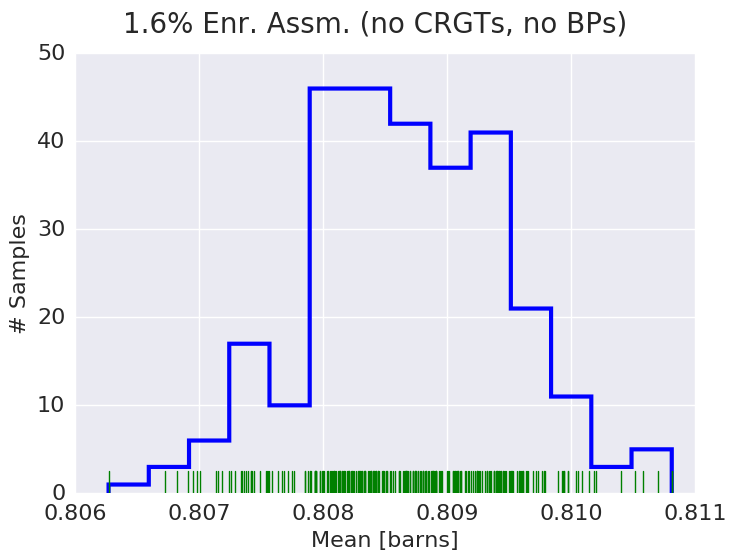
\includegraphics[width=\linewidth]{figures/patterns/assm-1.6-inf/hist-kde-rug/assm-16-inf-capt-1}
  \caption{}
  \label{fig:chap9-hist-assm-1.6-inf-capt}
\end{subfigure}%
\begin{subfigure}{0.5\textwidth}
  \centering
  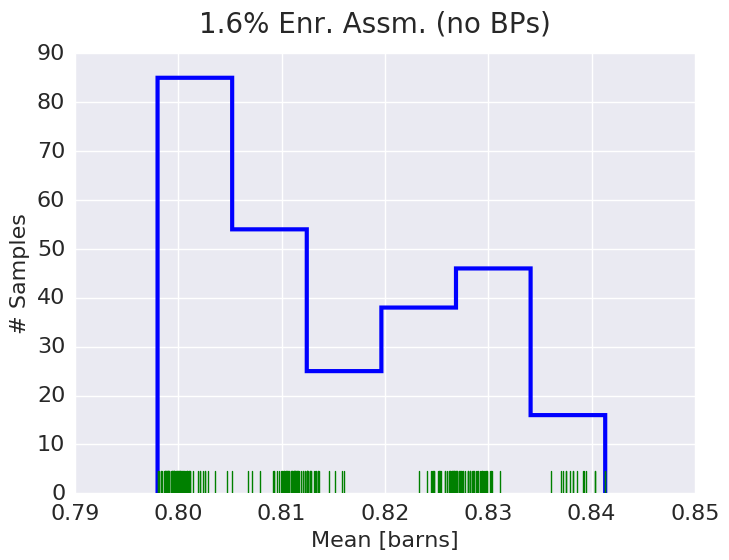
\includegraphics[width=\linewidth]{figures/patterns/assm-1.6/hist-kde-rug/assm-16-capt-1}
  \caption{}
  \label{fig:chap9-hist-assm-1.6-capt}
\end{subfigure}
\begin{subfigure}{0.5\textwidth}
  \centering
  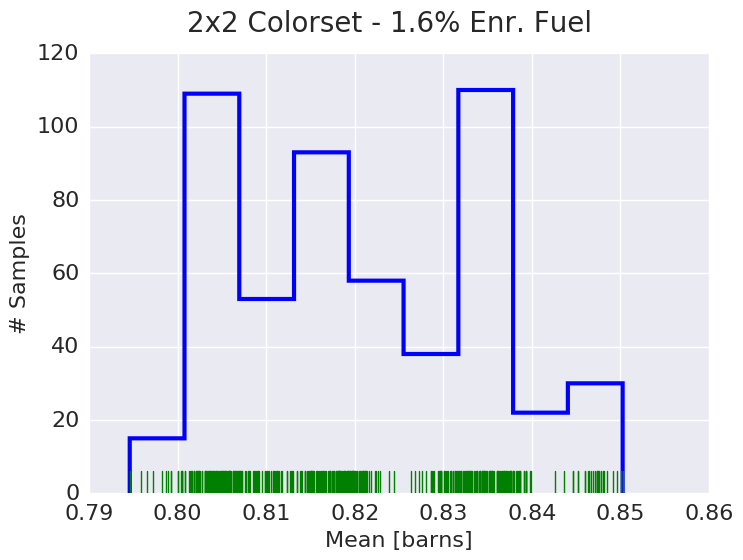
\includegraphics[width=\linewidth]{figures/patterns/2x2/hist-kde-rug/16-enr-capt-1}
  \caption{}
  \label{fig:chap9-hist-2x2-1.6-capt}
\end{subfigure}%
\begin{subfigure}{0.5\textwidth}
  \centering
  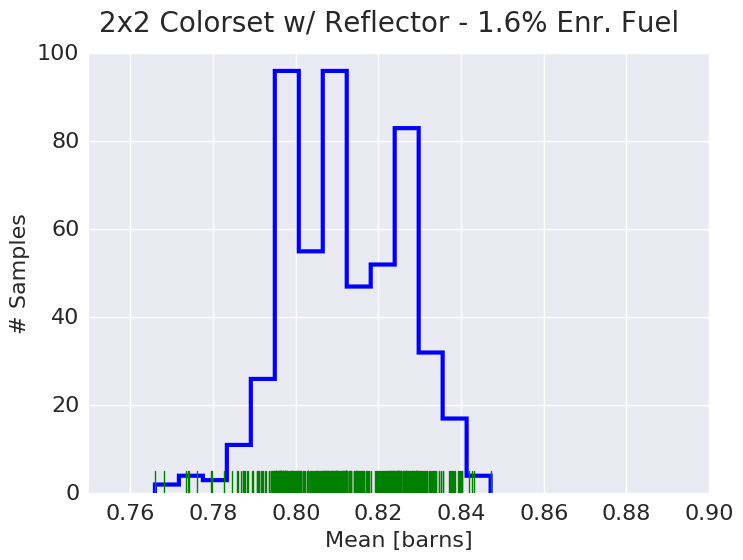
\includegraphics[width=\linewidth]{figures/patterns/reflector/hist-kde-rug/16-enr-capt-1}  \caption{}
  \label{fig:chap9-hist-reflector-1.6-capt}
\end{subfigure}
\begin{subfigure}{0.5\textwidth}
  \centering
  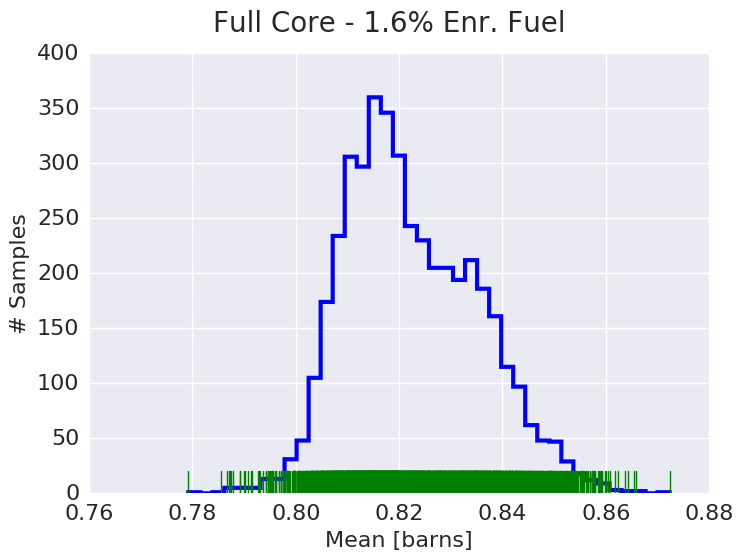
\includegraphics[width=\linewidth]{figures/patterns/full-core/hist-kde-rug/16-enr-capt-1} \caption{}
  \label{fig:chap9-hist-full-core-1.6-capt}
\end{subfigure}
\caption[Histogram of U-238 capture MGXS for 1.6\% enriched fuel]{Histograms of U-238 capture \ac{MGXS} for 1.6\% enriched fuel.}
\label{fig:chap9-hist-1.6-capt}
\end{figure}

\begin{figure}[h!]
\centering
\begin{subfigure}{0.5\textwidth}
  \centering
  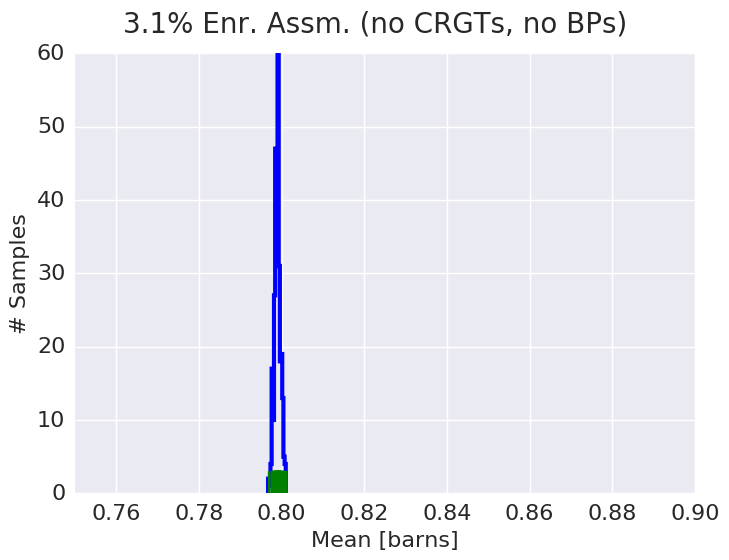
\includegraphics[width=\linewidth]{figures/patterns/assm-3.1-inf/hist-kde-rug/assm-31-inf-capt-1}
  \caption{}
  \label{fig:chap9-hist-assm-3.1-inf-capt}
\end{subfigure}%
\begin{subfigure}{0.5\textwidth}
  \centering
  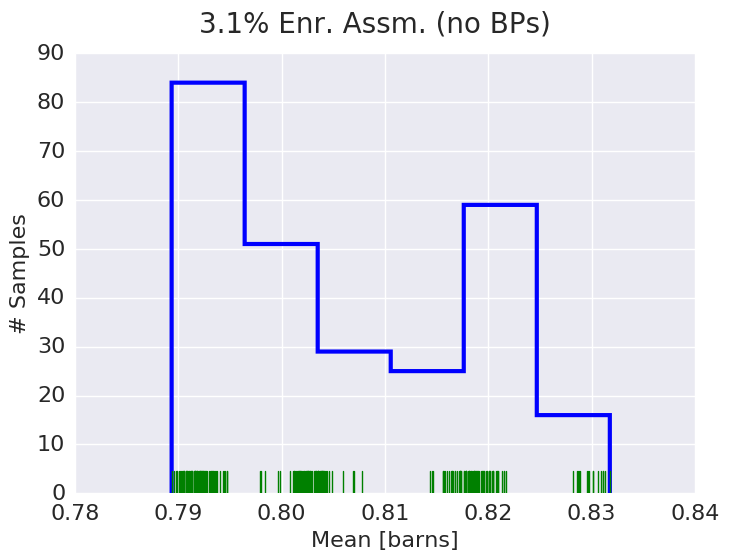
\includegraphics[width=\linewidth]{figures/patterns/assm-3.1/hist-kde-rug/assm-31-capt-1}
  \caption{}
  \label{fig:chap9-hist-assm-3.1-capt}
\end{subfigure}
\begin{subfigure}{0.5\textwidth}
  \centering
  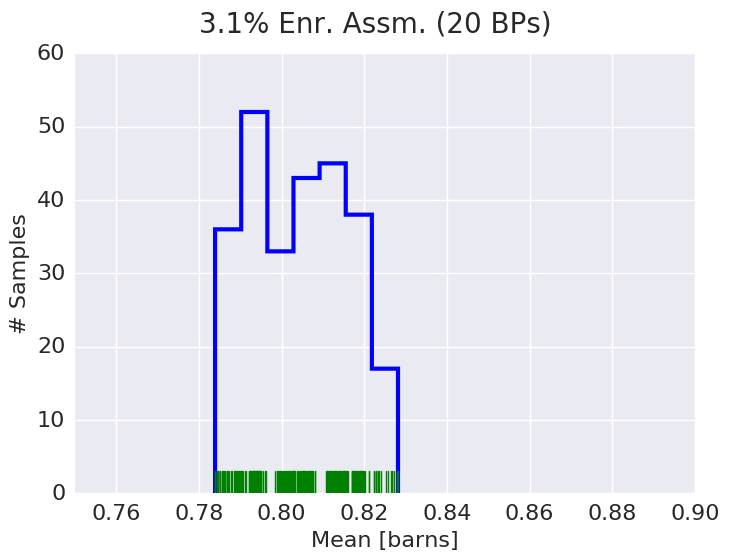
\includegraphics[width=\linewidth]{figures/patterns/assm-3.1-20BPs/hist-kde-rug/assm-31-20BPs-capt-1}
  \caption{}
  \label{fig:chap9-hist-assm-3.1-20BPs-capt}
\end{subfigure}%
\begin{subfigure}{0.5\textwidth}
  \centering
  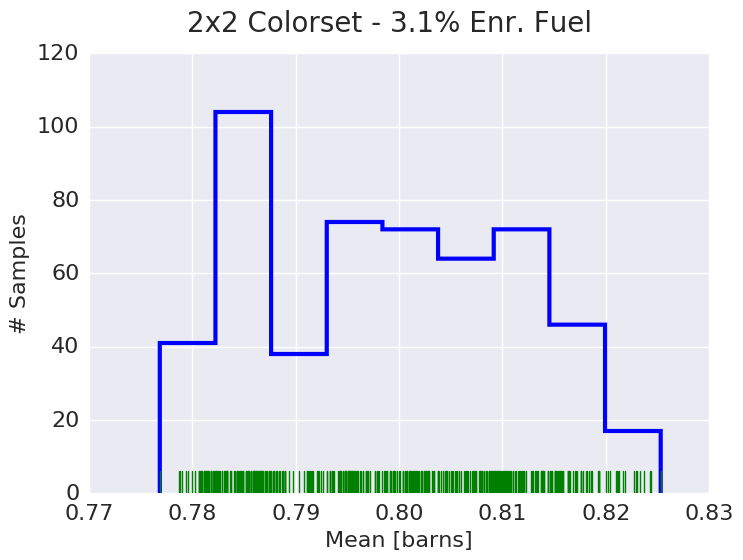
\includegraphics[width=\linewidth]{figures/patterns/2x2/hist-kde-rug/31-enr-capt-1}
  \caption{}
  \label{fig:chap9-hist-2x2-3.1-capt}
\end{subfigure}
\begin{subfigure}{0.5\textwidth}
  \centering
  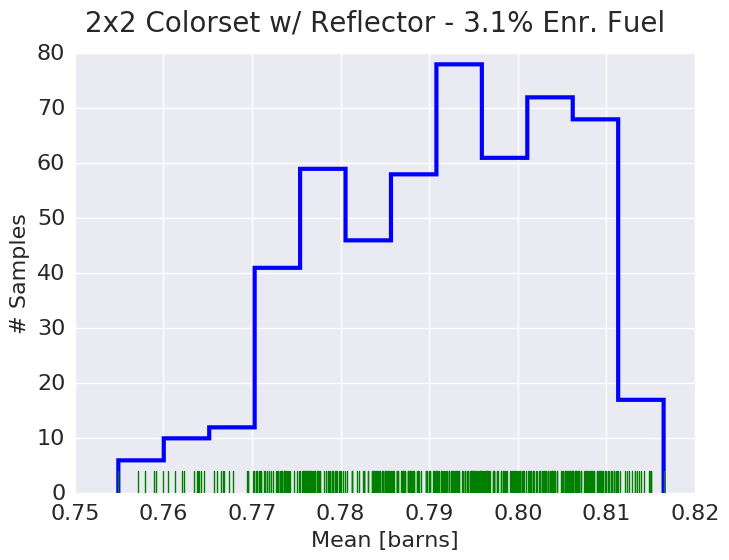
\includegraphics[width=\linewidth]{figures/patterns/reflector/hist-kde-rug/31-enr-capt-1}  \caption{}
  \label{fig:chap9-hist-reflector-3.1-capt}
\end{subfigure}%
\begin{subfigure}{0.5\textwidth}
  \centering
  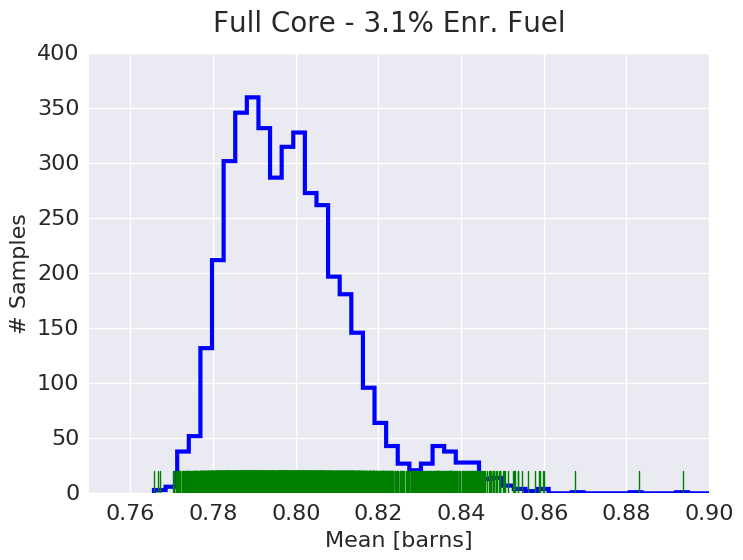
\includegraphics[width=\linewidth]{figures/patterns/full-core/hist-kde-rug/31-enr-capt-1} \caption{}
  \label{fig:chap9-hist-full-core-3.1-capt}
\end{subfigure}
\caption[Histogram of U-238 capture MGXS for 3.1\% enriched fuel]{Histograms of U-238 capture \ac{MGXS} for 3.1\% enriched fuel.}
\label{fig:chap9-hist-3.1-capt}
\end{figure}


\begin{figure}[h!]
\centering
\begin{subfigure}{0.5\textwidth}
  \centering
  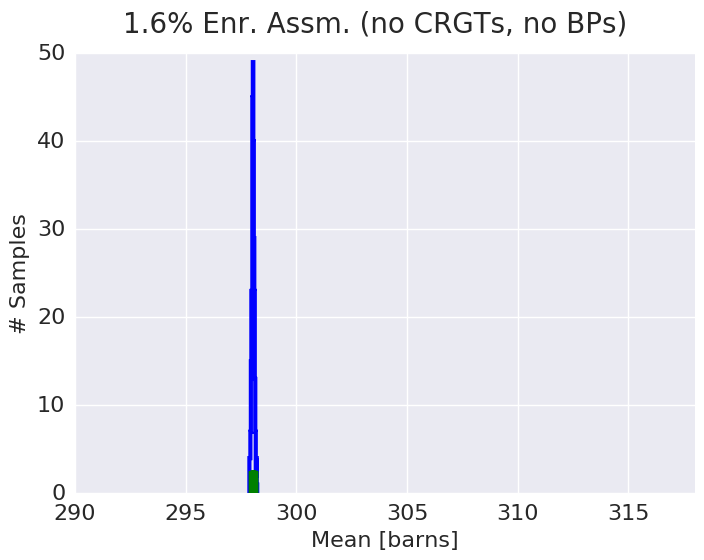
\includegraphics[width=\linewidth]{figures/patterns/assm-1.6-inf/hist-kde-rug/assm-16-inf-fiss-2}
  \caption{}
  \label{fig:chap9-hist-assm-1.6-inf-fiss}
\end{subfigure}%
\begin{subfigure}{0.5\textwidth}
  \centering
  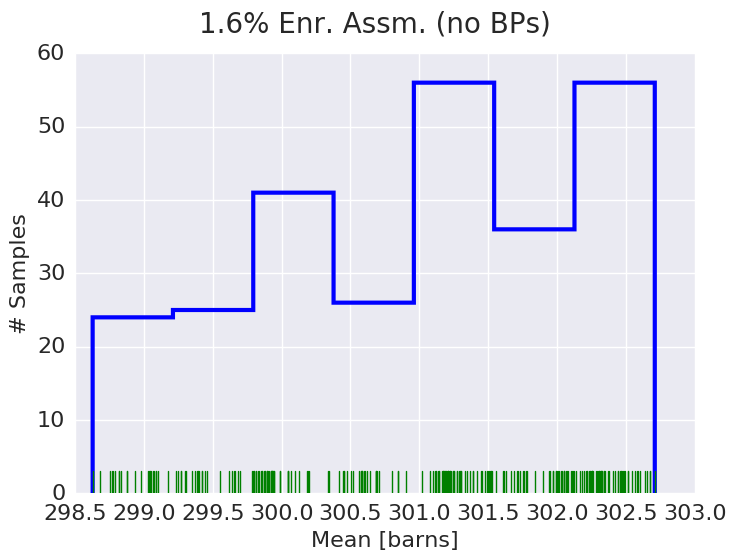
\includegraphics[width=\linewidth]{figures/patterns/assm-1.6/hist-kde-rug/assm-16-fiss-2}
  \caption{}
  \label{fig:chap9-hist-assm-1.6-fiss}
\end{subfigure}
\begin{subfigure}{0.5\textwidth}
  \centering
  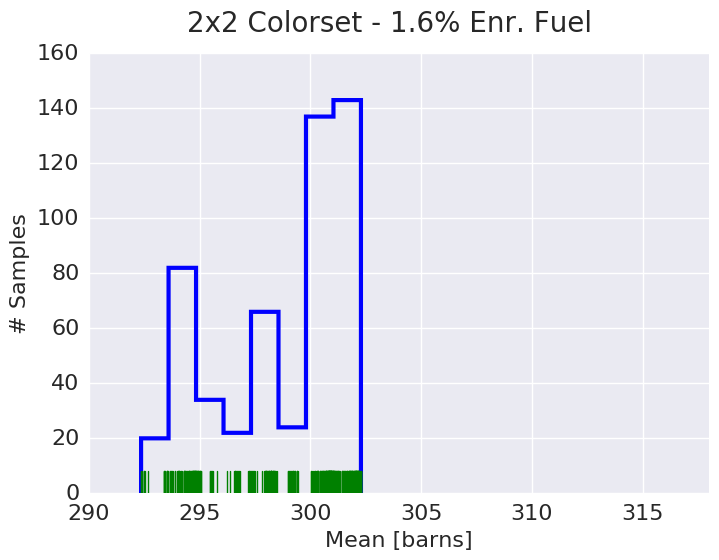
\includegraphics[width=\linewidth]{figures/patterns/2x2/hist-kde-rug/16-enr-fiss-2}
  \caption{}
  \label{fig:chap9-hist-2x2-1.6-fiss}
\end{subfigure}%
\begin{subfigure}{0.5\textwidth}
  \centering
  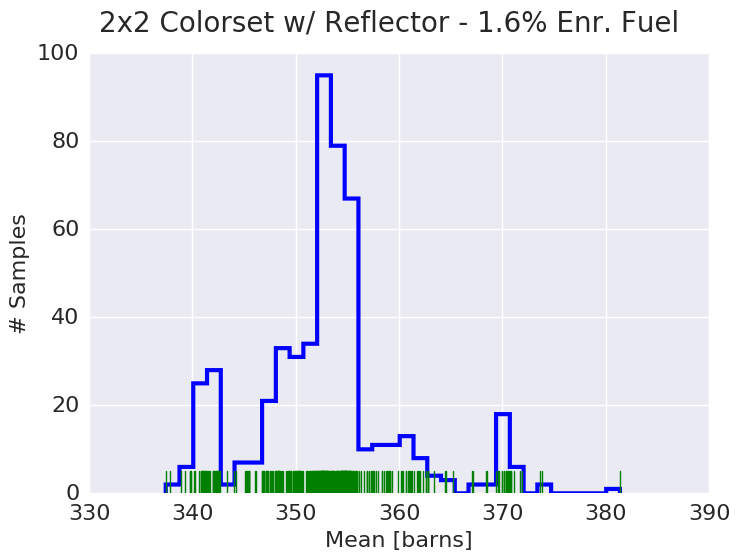
\includegraphics[width=\linewidth]{figures/patterns/reflector/hist-kde-rug/16-enr-fiss-2}  \caption{}
  \label{fig:chap9-hist-reflector-1.6-fiss}
\end{subfigure}
\begin{subfigure}{0.5\textwidth}
  \centering
  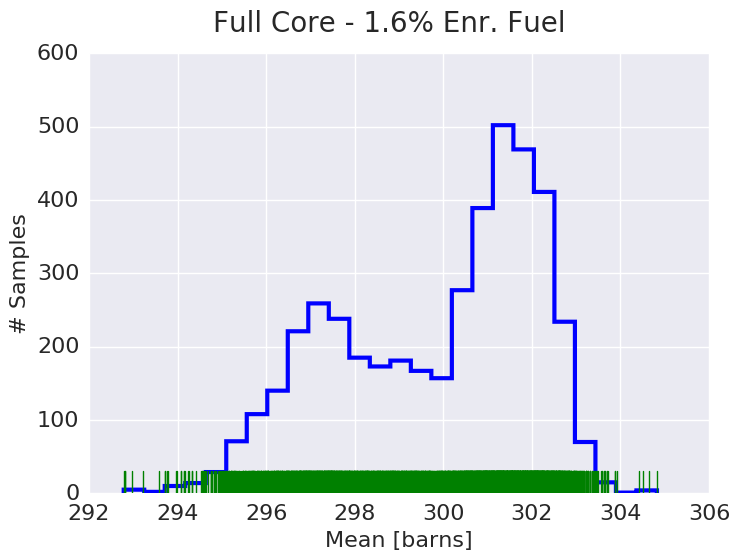
\includegraphics[width=\linewidth]{figures/patterns/full-core/hist-kde-rug/16-enr-fiss-2} \caption{}
  \label{fig:chap9-hist-full-core-1.6-fiss}
\end{subfigure}
\caption[Histogram of U-235 fission MGXS for 1.6\% enriched fuel]{Histograms of U-235 fission \ac{MGXS} for 1.6\% enriched fuel.}
\label{fig:chap9-hist-1.6-fiss}
\end{figure}

\begin{figure}[h!]
\centering
\begin{subfigure}{0.5\textwidth}
  \centering
  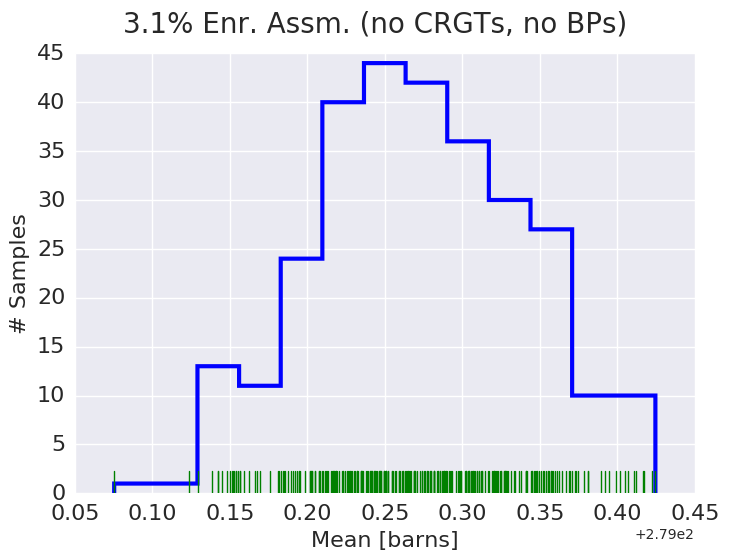
\includegraphics[width=\linewidth]{figures/patterns/assm-3.1-inf/hist-kde-rug/assm-31-inf-fiss-2}
  \caption{}
  \label{fig:chap9-hist-assm-3.1-inf-fiss}
\end{subfigure}%
\begin{subfigure}{0.5\textwidth}
  \centering
  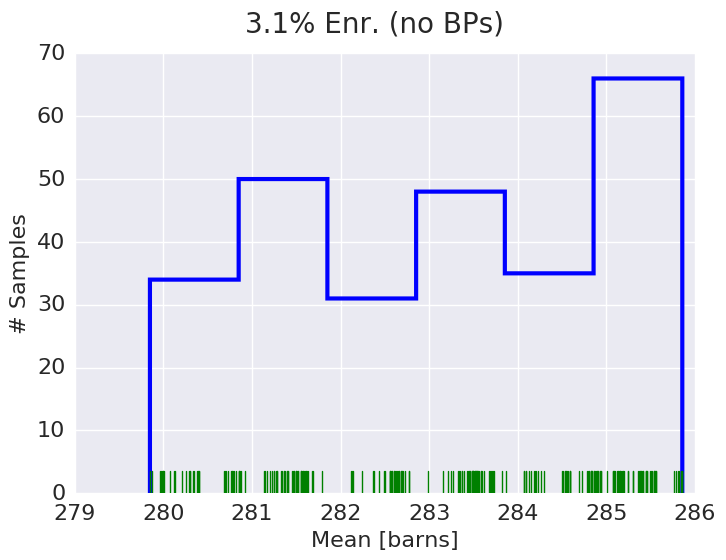
\includegraphics[width=\linewidth]{figures/patterns/assm-3.1/hist-kde-rug/assm-31-fiss-2}
  \caption{}
  \label{fig:chap9-hist-assm-3.1-fiss}
\end{subfigure}
\begin{subfigure}{0.5\textwidth}
  \centering
  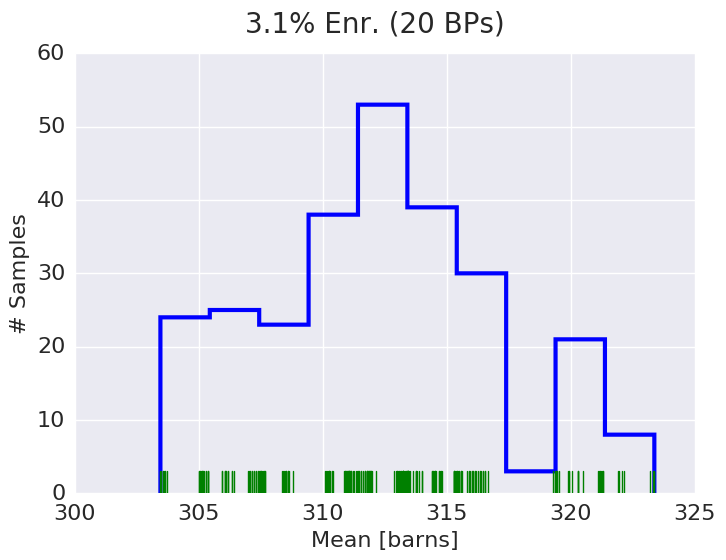
\includegraphics[width=\linewidth]{figures/patterns/assm-3.1-20BPs/hist-kde-rug/assm-31-20BPs-fiss-2}
  \caption{}
  \label{fig:chap9-hist-assm-3.1-20BPs-fiss}
\end{subfigure}%
\begin{subfigure}{0.5\textwidth}
  \centering
  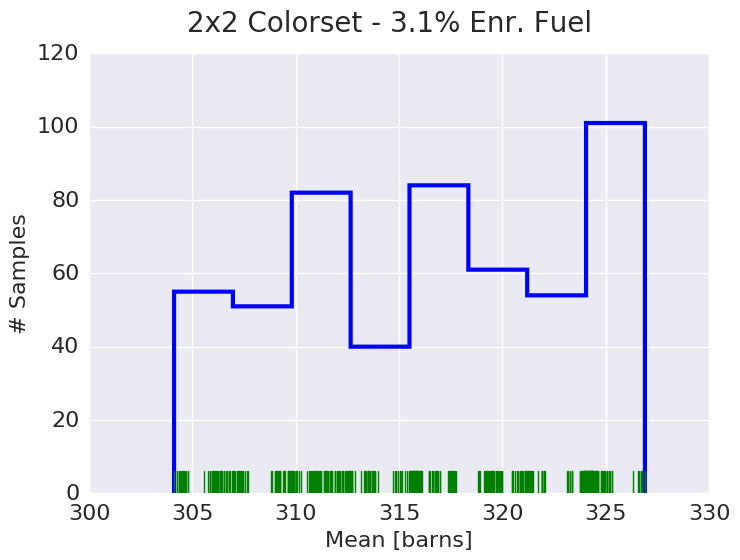
\includegraphics[width=\linewidth]{figures/patterns/2x2/hist-kde-rug/31-enr-fiss-2}
  \caption{}
  \label{fig:chap9-hist-2x2-3.1-fiss}
\end{subfigure}
\begin{subfigure}{0.5\textwidth}
  \centering
  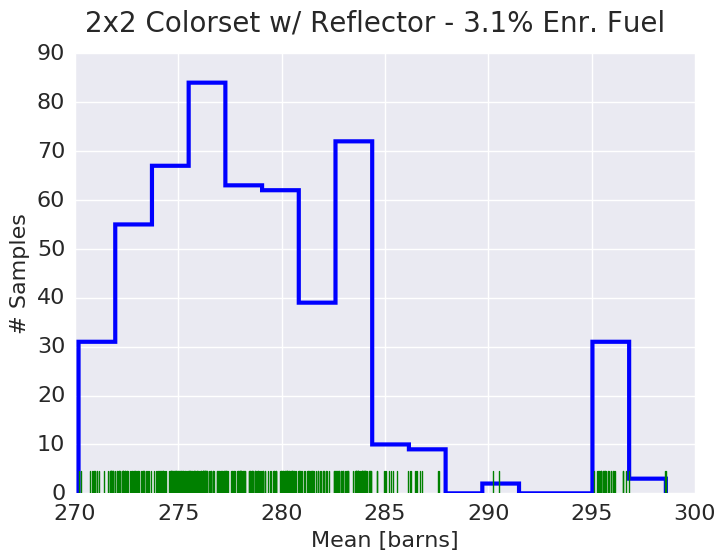
\includegraphics[width=\linewidth]{figures/patterns/reflector/hist-kde-rug/31-enr-fiss-2}  \caption{}
  \label{fig:chap9-hist-reflector-3.1-fiss}
\end{subfigure}%
\begin{subfigure}{0.5\textwidth}
  \centering
  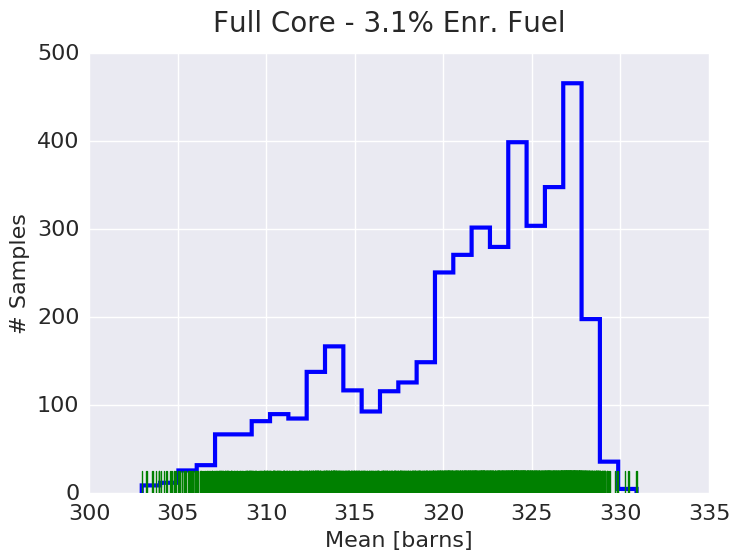
\includegraphics[width=\linewidth]{figures/patterns/full-core/hist-kde-rug/31-enr-fiss-2} \caption{}
  \label{fig:chap9-hist-full-core-3.1-fiss}
\end{subfigure}
\caption[Histogram of U-235 fission MGXS 3.1\% enriched fuel]{Histograms of U-235 fission \ac{MGXS} for 3.1\% enriched fuel.}
\label{fig:chap9-hist-3.1-fiss}
\end{figure}



\begin{figure}[h!]
\centering
\begin{subfigure}{0.5\textwidth}
  \centering
  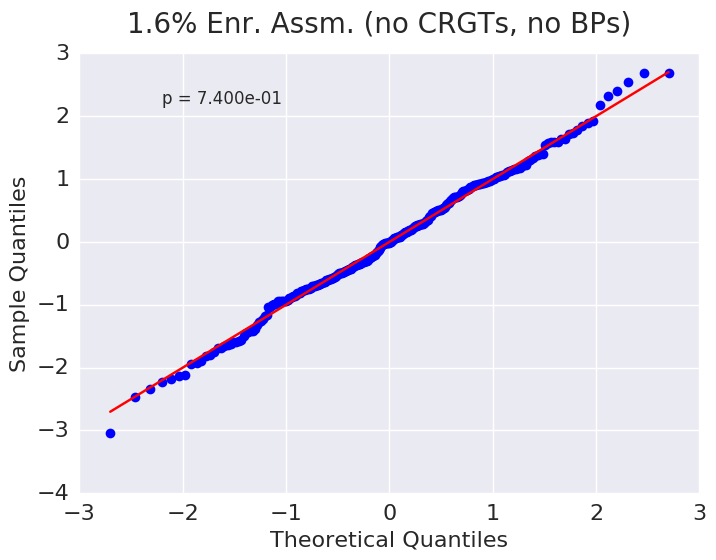
\includegraphics[width=\linewidth]{figures/patterns/assm-1.6-inf/quantile/assm-16-inf-capt-1}
  \caption{}
  \label{fig:chap9-qq-assm-1.6-inf-capt}
\end{subfigure}%
\begin{subfigure}{0.5\textwidth}
  \centering
  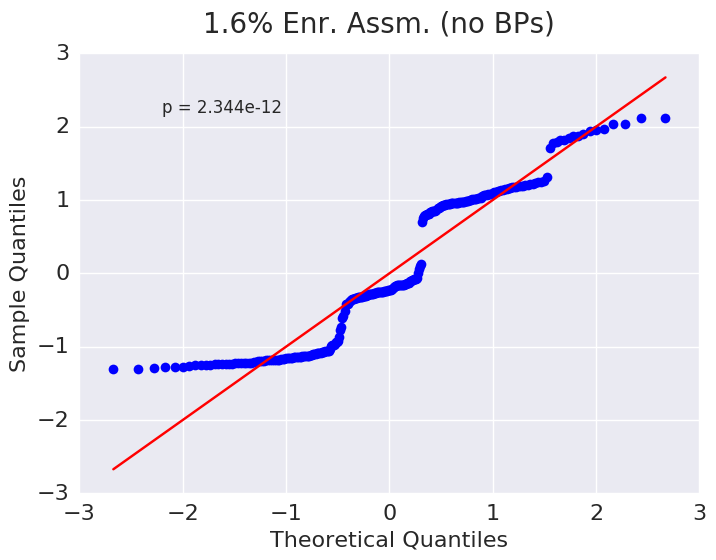
\includegraphics[width=\linewidth]{figures/patterns/assm-1.6/quantile/assm-16-capt-1}
  \caption{}
  \label{fig:chap9-qq-assm-1.6-capt}
\end{subfigure}
\begin{subfigure}{0.5\textwidth}
  \centering
  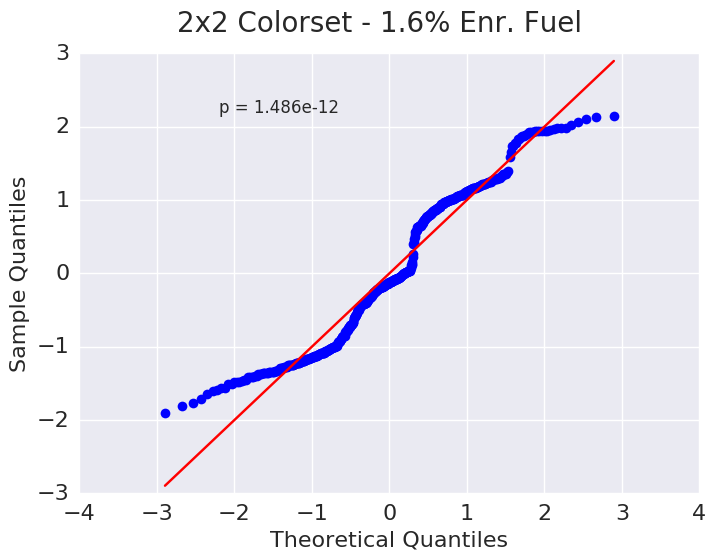
\includegraphics[width=\linewidth]{figures/patterns/2x2/quantile/16-enr-capt-1}
  \caption{}
  \label{fig:chap9-qq-2x2-1.6-capt}
\end{subfigure}%
\begin{subfigure}{0.5\textwidth}
  \centering
  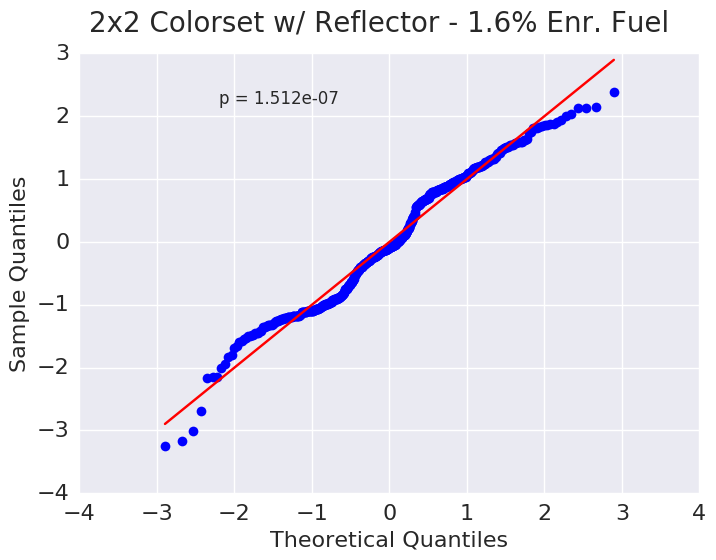
\includegraphics[width=\linewidth]{figures/patterns/reflector/quantile/16-enr-capt-1}  \caption{}
  \label{fig:chap9-qq-reflector-1.6-capt}
\end{subfigure}
\begin{subfigure}{0.5\textwidth}
  \centering
  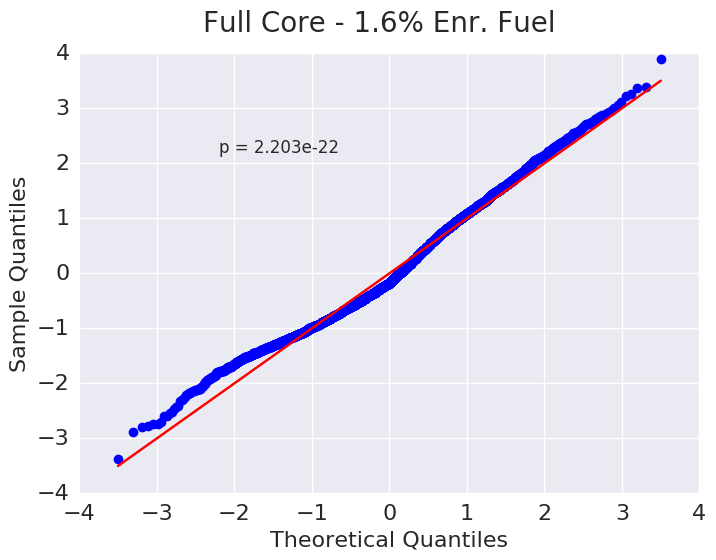
\includegraphics[width=\linewidth]{figures/patterns/full-core/quantile/16-enr-capt-1} \caption{}
  \label{fig:chap9-qq-full-core-1.6-capt}
\end{subfigure}
\caption[Q-Q plots of U-238 capture MGXS for 1.6\% enriched fuel]{Q-Q plots of U-238 capture \ac{MGXS} for 1.6\% enriched fuel.}
\label{fig:chap9-qq-1.6-capt}
\end{figure}

\begin{figure}[h!]
\centering
\begin{subfigure}{0.5\textwidth}
  \centering
  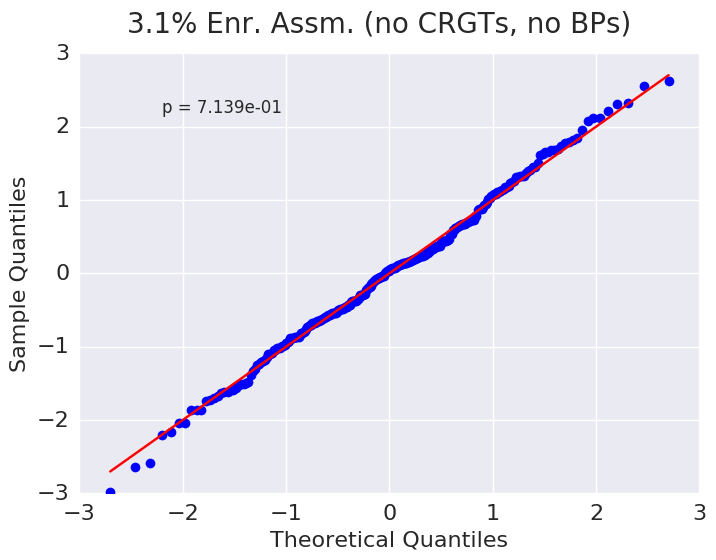
\includegraphics[width=\linewidth]{figures/patterns/assm-3.1-inf/quantile/assm-31-inf-capt-1}
  \caption{}
  \label{fig:chap9-qq-assm-3.1-inf-capt}
\end{subfigure}%
\begin{subfigure}{0.5\textwidth}
  \centering
  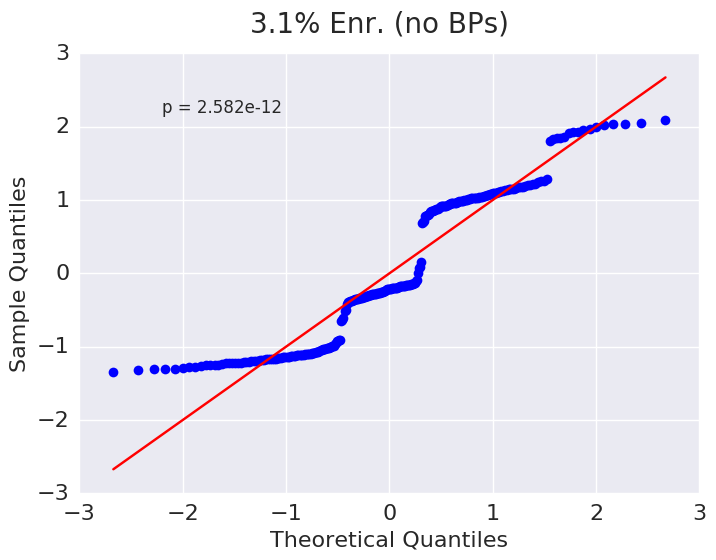
\includegraphics[width=\linewidth]{figures/patterns/assm-3.1/quantile/assm-31-capt-1}
  \caption{}
  \label{fig:chap9-qq-assm-3.1-capt}
\end{subfigure}
\begin{subfigure}{0.5\textwidth}
  \centering
  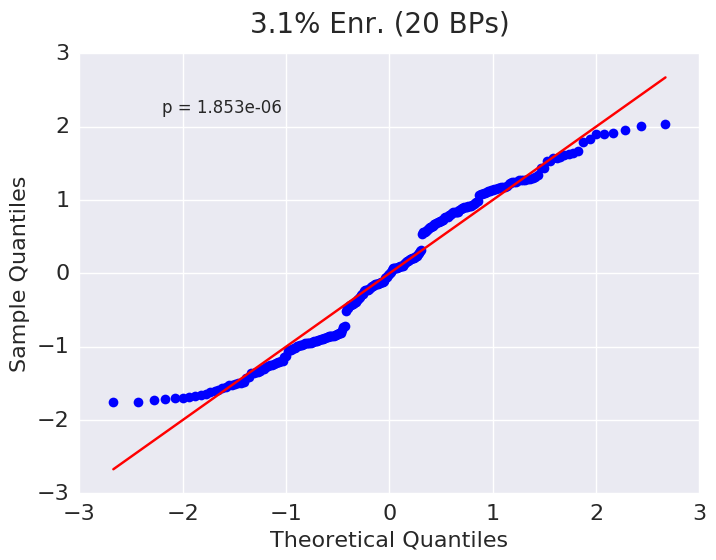
\includegraphics[width=\linewidth]{figures/patterns/assm-3.1-20BPs/quantile/assm-31-20BPs-capt-1}
  \caption{}
  \label{fig:chap9-qq-assm-3.1-20BPs-capt}
\end{subfigure}%
\begin{subfigure}{0.5\textwidth}
  \centering
  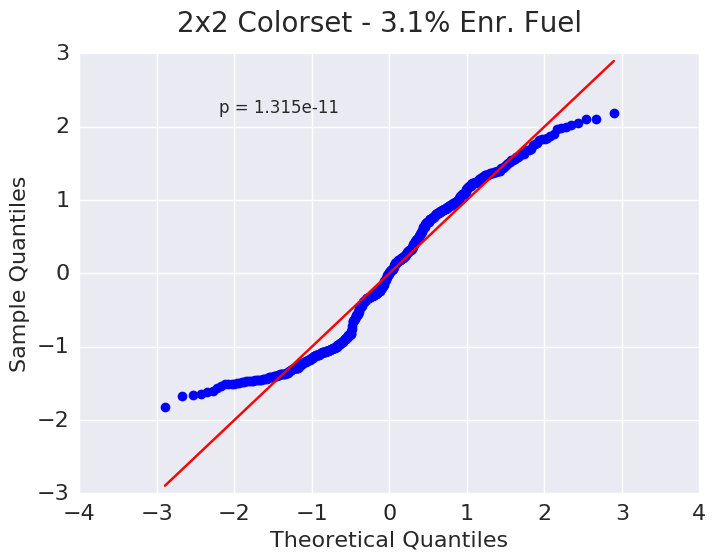
\includegraphics[width=\linewidth]{figures/patterns/2x2/quantile/31-enr-capt-1}
  \caption{}
  \label{fig:chap9-qq-2x2-3.1-capt}
\end{subfigure}
\begin{subfigure}{0.5\textwidth}
  \centering
  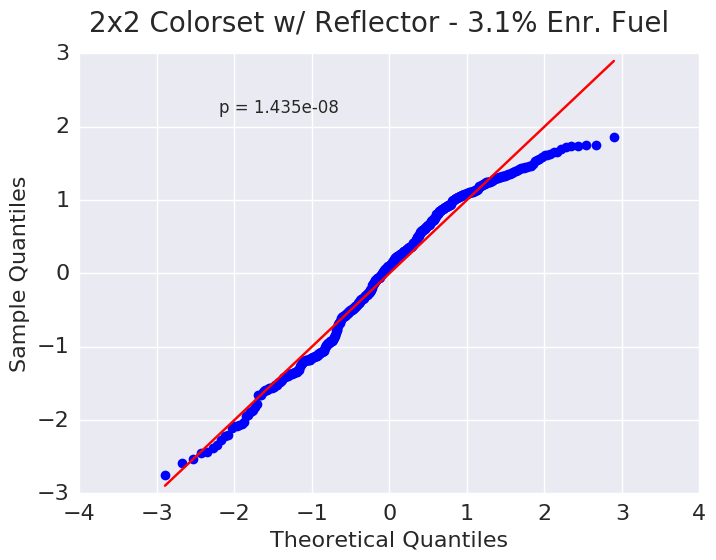
\includegraphics[width=\linewidth]{figures/patterns/reflector/quantile/31-enr-capt-1}  \caption{}
  \label{fig:chap9-qq-reflector-3.1-capt}
\end{subfigure}%
\begin{subfigure}{0.5\textwidth}
  \centering
  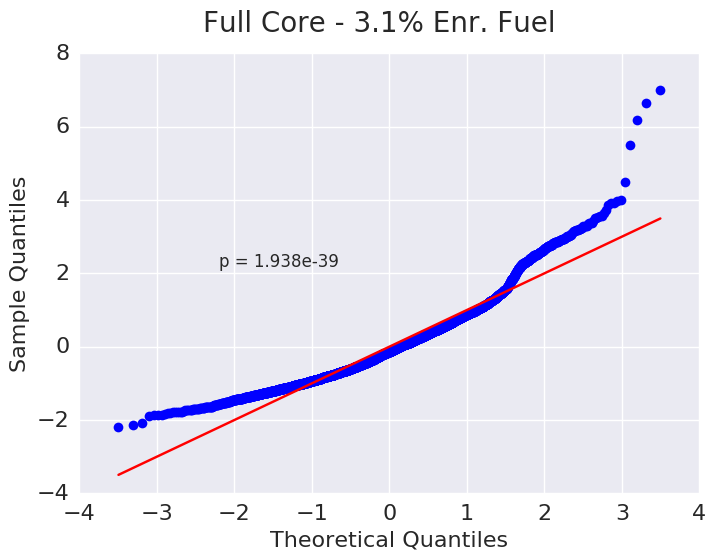
\includegraphics[width=\linewidth]{figures/patterns/full-core/quantile/31-enr-capt-1} \caption{}
  \label{fig:chap9-qq-full-core-3.1-capt}
\end{subfigure}
\caption[Q-Q plots of U-238 capture MGXS for 3.1\% enriched fuel]{Q-Q plots of U-238 capture \ac{MGXS} for 3.1\% enriched fuel.}
\label{fig:chap9-qq-3.1-capt}
\end{figure}


\begin{figure}[h!]
\centering
\begin{subfigure}{0.5\textwidth}
  \centering
  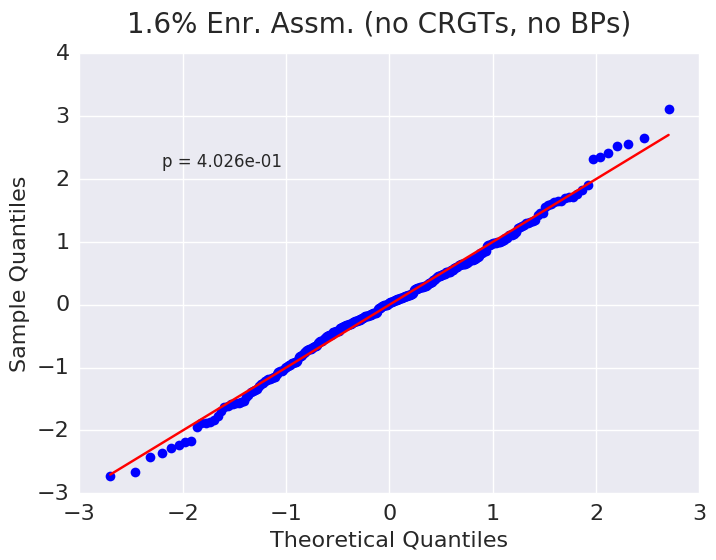
\includegraphics[width=\linewidth]{figures/patterns/assm-1.6-inf/quantile/assm-16-inf-fiss-2}
  \caption{}
  \label{fig:chap9-qq-assm-1.6-inf-fiss}
\end{subfigure}%
\begin{subfigure}{0.5\textwidth}
  \centering
  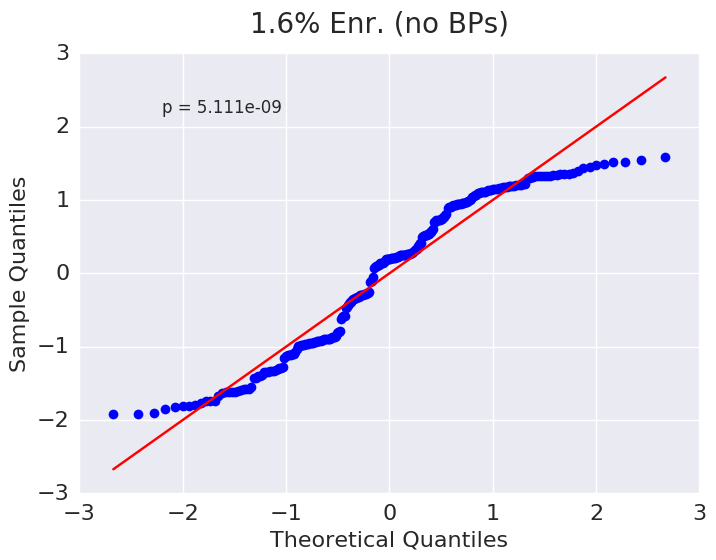
\includegraphics[width=\linewidth]{figures/patterns/assm-1.6/quantile/assm-16-fiss-2}
  \caption{}
  \label{fig:chap9-qq-assm-1.6-fiss}
\end{subfigure}
\begin{subfigure}{0.5\textwidth}
  \centering
  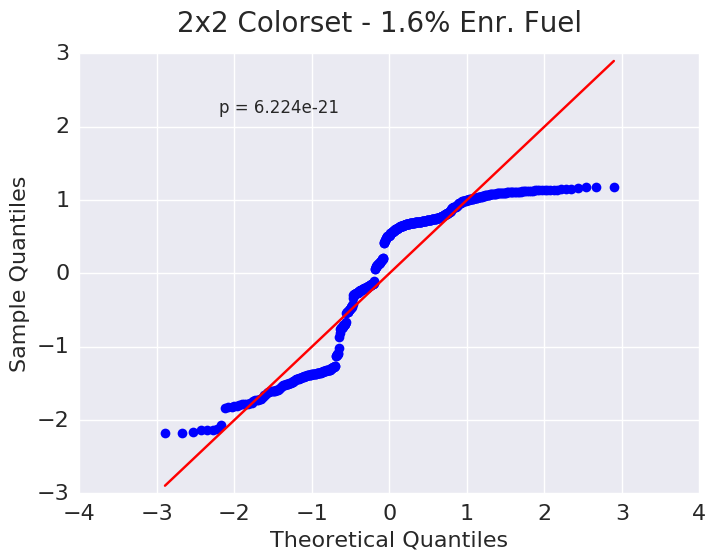
\includegraphics[width=\linewidth]{figures/patterns/2x2/quantile/16-enr-fiss-2}
  \caption{}
  \label{fig:chap9-qq-2x2-1.6-fiss}
\end{subfigure}%
\begin{subfigure}{0.5\textwidth}
  \centering
  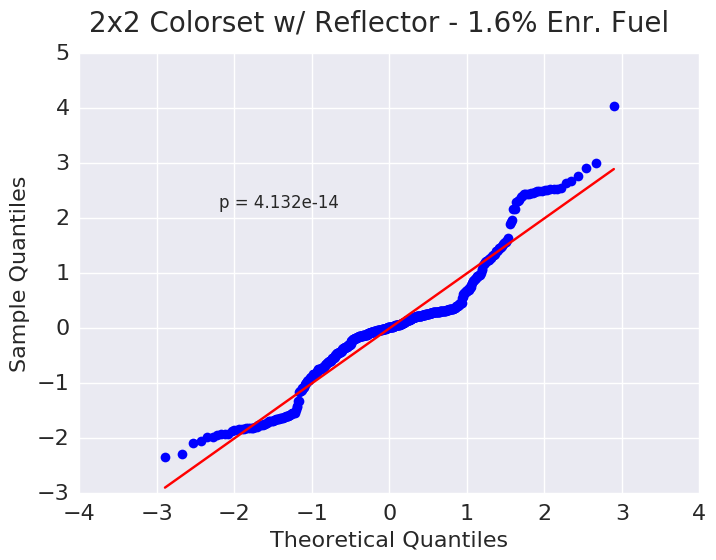
\includegraphics[width=\linewidth]{figures/patterns/reflector/quantile/16-enr-fiss-2}  \caption{}
  \label{fig:chap9-qq-reflector-1.6-fiss}
\end{subfigure}
\begin{subfigure}{0.5\textwidth}
  \centering
  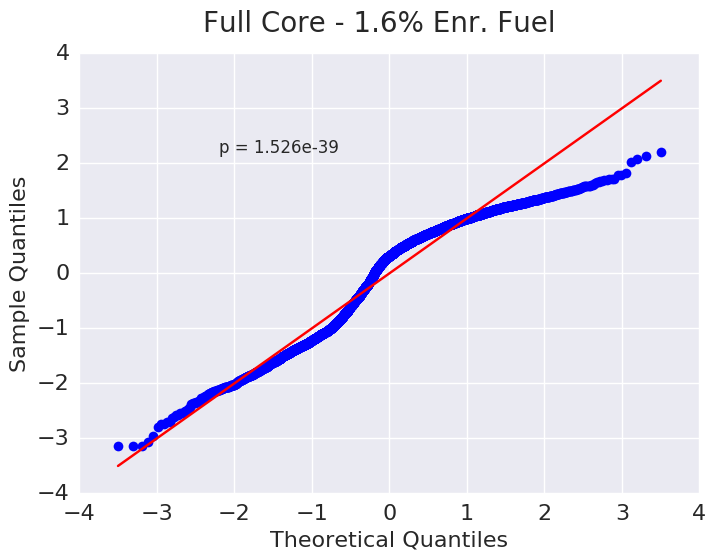
\includegraphics[width=\linewidth]{figures/patterns/full-core/quantile/16-enr-fiss-2} \caption{}
  \label{fig:chap9-qq-full-core-1.6-fiss}
\end{subfigure}
\caption[Q-Q plots of U-235 fission MGXS for 1.6\% enriched fuel]{Q-Q plots of U-235 fission \ac{MGXS} for 1.6\% enriched fuel.}
\label{fig:chap9-qq-1.6-fiss}
\end{figure}

\begin{figure}[h!]
\centering
\begin{subfigure}{0.5\textwidth}
  \centering
  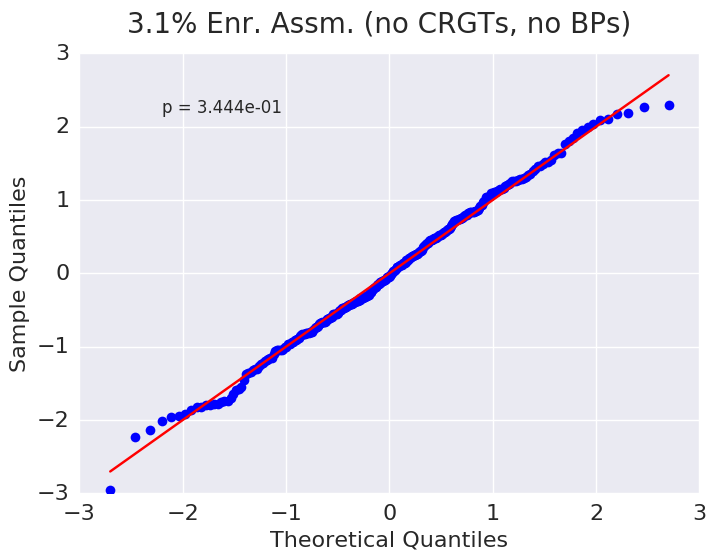
\includegraphics[width=\linewidth]{figures/patterns/assm-3.1-inf/quantile/assm-31-inf-fiss-2}
  \caption{}
  \label{fig:chap9-qq-assm-3.1-inf-fiss}
\end{subfigure}%
\begin{subfigure}{0.5\textwidth}
  \centering
  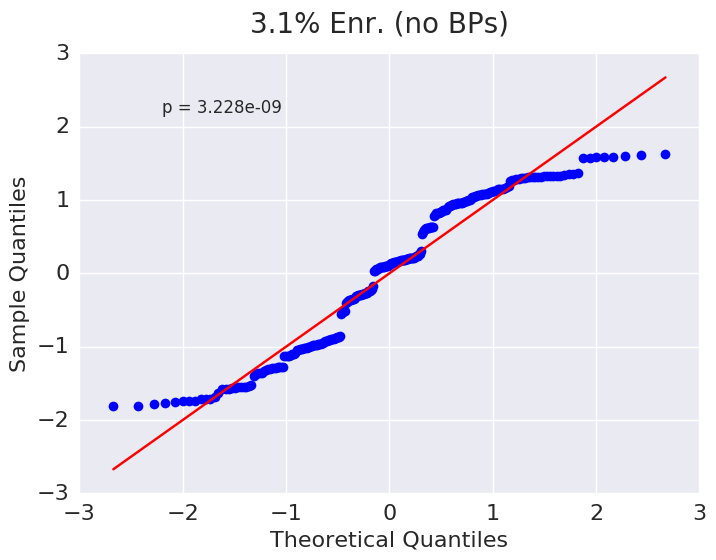
\includegraphics[width=\linewidth]{figures/patterns/assm-3.1/quantile/assm-31-fiss-2}
  \caption{}
  \label{fig:chap9-qq-assm-3.1-fiss}
\end{subfigure}
\begin{subfigure}{0.5\textwidth}
  \centering
  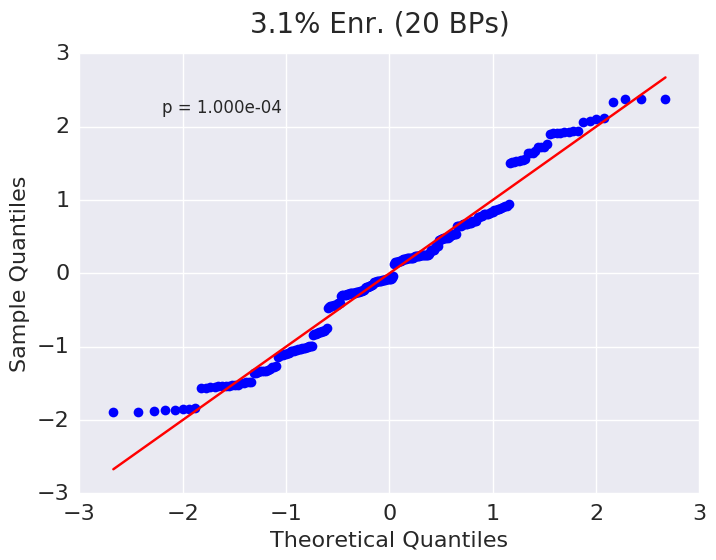
\includegraphics[width=\linewidth]{figures/patterns/assm-3.1-20BPs/quantile/assm-31-20BPs-fiss-2}
  \caption{}
  \label{fig:chap9-qq-assm-3.1-20BPs-fiss}
\end{subfigure}%
\begin{subfigure}{0.5\textwidth}
  \centering
  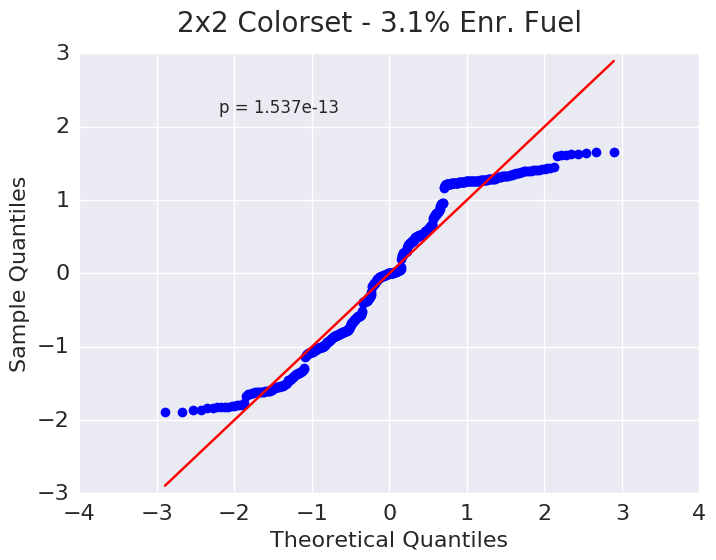
\includegraphics[width=\linewidth]{figures/patterns/2x2/quantile/31-enr-fiss-2}
  \caption{}
  \label{fig:chap9-qq-2x2-3.1-fiss}
\end{subfigure}
\begin{subfigure}{0.5\textwidth}
  \centering
  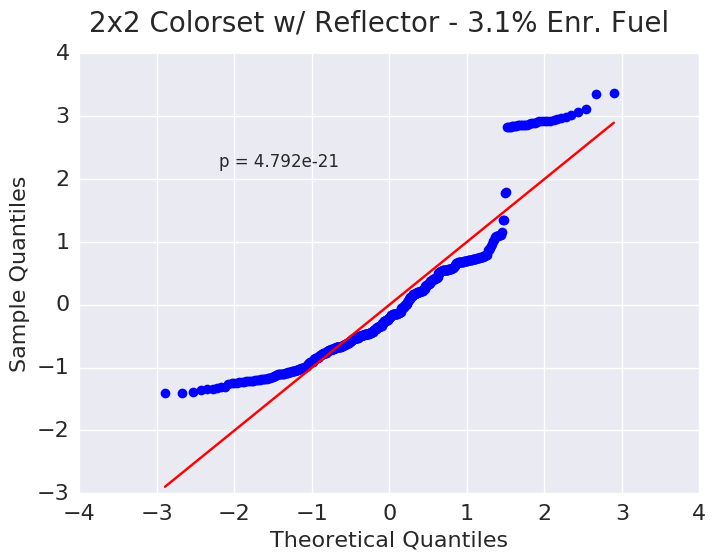
\includegraphics[width=\linewidth]{figures/patterns/reflector/quantile/31-enr-fiss-2}  \caption{}
  \label{fig:chap9-qq-reflector-3.1-fiss}
\end{subfigure}%
\begin{subfigure}{0.5\textwidth}
  \centering
  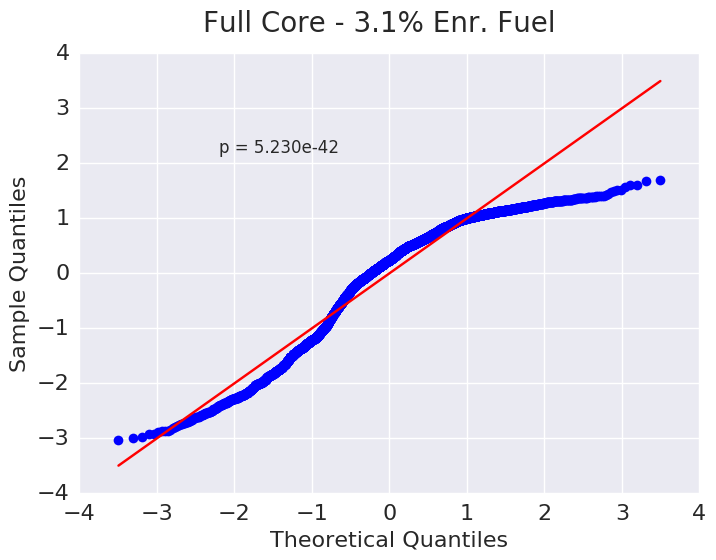
\includegraphics[width=\linewidth]{figures/patterns/full-core/quantile/31-enr-fiss-2} \caption{}
  \label{fig:chap9-qq-full-core-3.1-fiss}
\end{subfigure}
\caption[Q-Q plots of U-235 fission MGXS 3.1\% enriched fuel]{Q-Q plots of U-235 fission \ac{MGXS} for 3.1\% enriched fuel.}
\label{fig:chap9-qq-3.1-fiss}
\end{figure}


\begin{table}[h!]
  \centering
  \caption[Population variance for pin-wise MGXS]{The population variance for pin-wise fission and U-238 capture \ac{MGXS}.}
  \small
  \label{table:chap9-pop-var-mgxs}
  \vspace{6pt}
  \begin{tabular}{C{2.5cm} l C{2.5cm} C{2.5cm}}
  \toprule
  \rowcolor{lightgray}
  \multicolumn{1}{C{2.5cm}}{\textbf{Fuel Enrichment}} & \multicolumn{1}{c}{\textbf{Benchmark}} & \boldmath$\mathrm{Var}\left[\sigma_{c}^{U-238}\right]$ \textbf{[barns]} & \boldmath$\mathrm{Var}\left[\sigma_{f}\right]$ \textbf{[barns]} \\
  \toprule
%  \multicolumn{3}{c}{\cellcolor{lightgray} \bf 1.6\% Enr. Fuel} \\
%\midrule
\multirow{5}{*}{1.6\%} & Assm. (no \acp{CRGT}, no \acp{BP}) & 6.29E-07 & 5.06E--03 \\
%\midrule
& Assm. (no \acp{BP}) & 1.61E-04 & 1.81E+00 \\
%\midrule
& 2$\times$2 Colorset & 1.89E-04 & 1.18E+01 \\
%\midrule
& 2$\times$2 Colorset w/ Reflector & 2.03E-04 & 1.93E+01 \\
%\midrule
& \ac{BEAVRS} Quarter Core & 1.64E-04 & 6.78E+00 \\
%\midrule
%\multicolumn{3}{c}{\cellcolor{lightgray} \bf 3.1\% Enr. Fuel} \\
\midrule
\multirow{6}{*}{3.1\%} & Assm. (no \acp{CRGT}, no \acp{BP}) & 5.83E-07 & 6.12E--03 \\
% \midrule
& Assm. (no \acp{BP}) & 1.53E-04 & 4.22E+00 \\
% \midrule
& Assm. (20 \acp{BP}) & 1.37E-04 & 1.11E+01 \\
% \midrule
& 2$\times$2 Colorset & 1.53E-04 & 2.15E+01 \\
% \midrule
& 2$\times$2 Colorset w/ Reflector & 1.79E-04 & 4.78E+01 \\
% \midrule
& \ac{BEAVRS} Quarter Core & 2.34E-04 & 1.68E+01 \\
\bottomrule
\end{tabular}
\end{table}


first paragraph:
-

second paragraph:
-

%\begin{itemize}[noitemsep]
%  \item show that clustering exists in MGXS
%  \begin{itemize}[noitemsep]
%    \item leave ``features'' and ML discussion for next chapter
%  \end{itemize}
%  \item look at slides 66-71 in ORNL presentation
%\end{itemize}


%%%%%%%%%%%%%%%%%%%%%%%%%%%%%%%%%%%%%%%%%%%%%%%%%%%%%%%%%%%%%%%%%%%%%%%%%%%%%%%
\section{Pin-Wise Population Variance}

-plot the convergence of null MGXS by batch along with max for distribcell MGXS
-plot the pop. var. convergence of the distribcell MGXS and show that they don't go to zero
-plot the convergence of the distribcell MGXS for 1.6\% enr. assm, 3.1\% assm w/ BPs, 2x2 colorset w/ reflector???

\begin{itemize}[noitemsep]
  \item table of population variance of distribcell MGXS
  \item plots of convergence of pop. var. of distribell MGXS
  \begin{itemize}[noitemsep]
    \item MGXS in moderator and fuel
    \item pop. var. in fuel converges to non-zero value
    \item pop. var. in moderator is negligible
  \end{itemize}
\end{itemize}


%%%%%%%%%%%%%%%%%%%%%%%%%%%%%%%%%%%%%%%%%%%%%%%%%%%%%%%%%%%%%%%%%%%%%%%%%%%%%%%
\section{Clustering MGXS with Local Neighbor Symmetry}

-need to define \ac{LNS} spatial homogenization
-refer back to workflow chapter and OpenCG

-boxplots / violin plots of MGXS for each???
-improved errors wrt. null homogenization

\begin{itemize}[noitemsep]
  \item objective is to capture clustering effects in MGXS
  \item introduce LNS algorithm, or reference from section on OpenCG
  \item LNS isn't adaptable -- segue to next chapter
\end{itemize}


\begin{table}[h!]
  \centering
  \caption[Number of materials for LNS spatial homogenization]{Number of materials modeled with unique \ac{MGXS} in each heterogeneous benchmark for \ac{LNS} spatial homogenization.}
  \small
  \label{table:chap9-num-materials-lns}
  \vspace{6pt}
  \begin{tabular}{l r r r}
  \toprule
  \rowcolor{lightgray}
  & \multicolumn{3}{c}{\cellcolor{lightgray} \bf \# Materials} \\
  \multirow{-2}{*}{\cellcolor{lightgray} \bf Benchmark} &
  \multicolumn{1}{c}{\cellcolor{lightgray} \bf Null/Infinite} &
  \multicolumn{1}{c}{\cellcolor{lightgray} \bf \ac{LNS}} &
  \multicolumn{1}{c}{\cellcolor{lightgray} \bf Degenerate} \\
  \midrule
1.6\% Assm & 5 & 13 & 268 \\
  \midrule
3.1\% Assm & 5 & 13 & 268 \\
  \midrule
3.1\% Assm w/ 20 BPs & 7 & 17 & 270  \\
  \midrule
2$\times$2 Colorset & 8 & 25 & 1,062 \\
  \midrule
2$\times$2 Colorset w/ Reflector & 8 & 35 & 1,062 \\
  \midrule
\ac{BEAVRS} Quarter Core & 10 & 497 & 13,000 \\ % LNS = ceil(193 / 4) * 10 + 7
  \bottomrule
\end{tabular}
\end{table}


\begin{figure}[h!]
\centering
\begin{subfigure}{.47\textwidth}
  \centering
  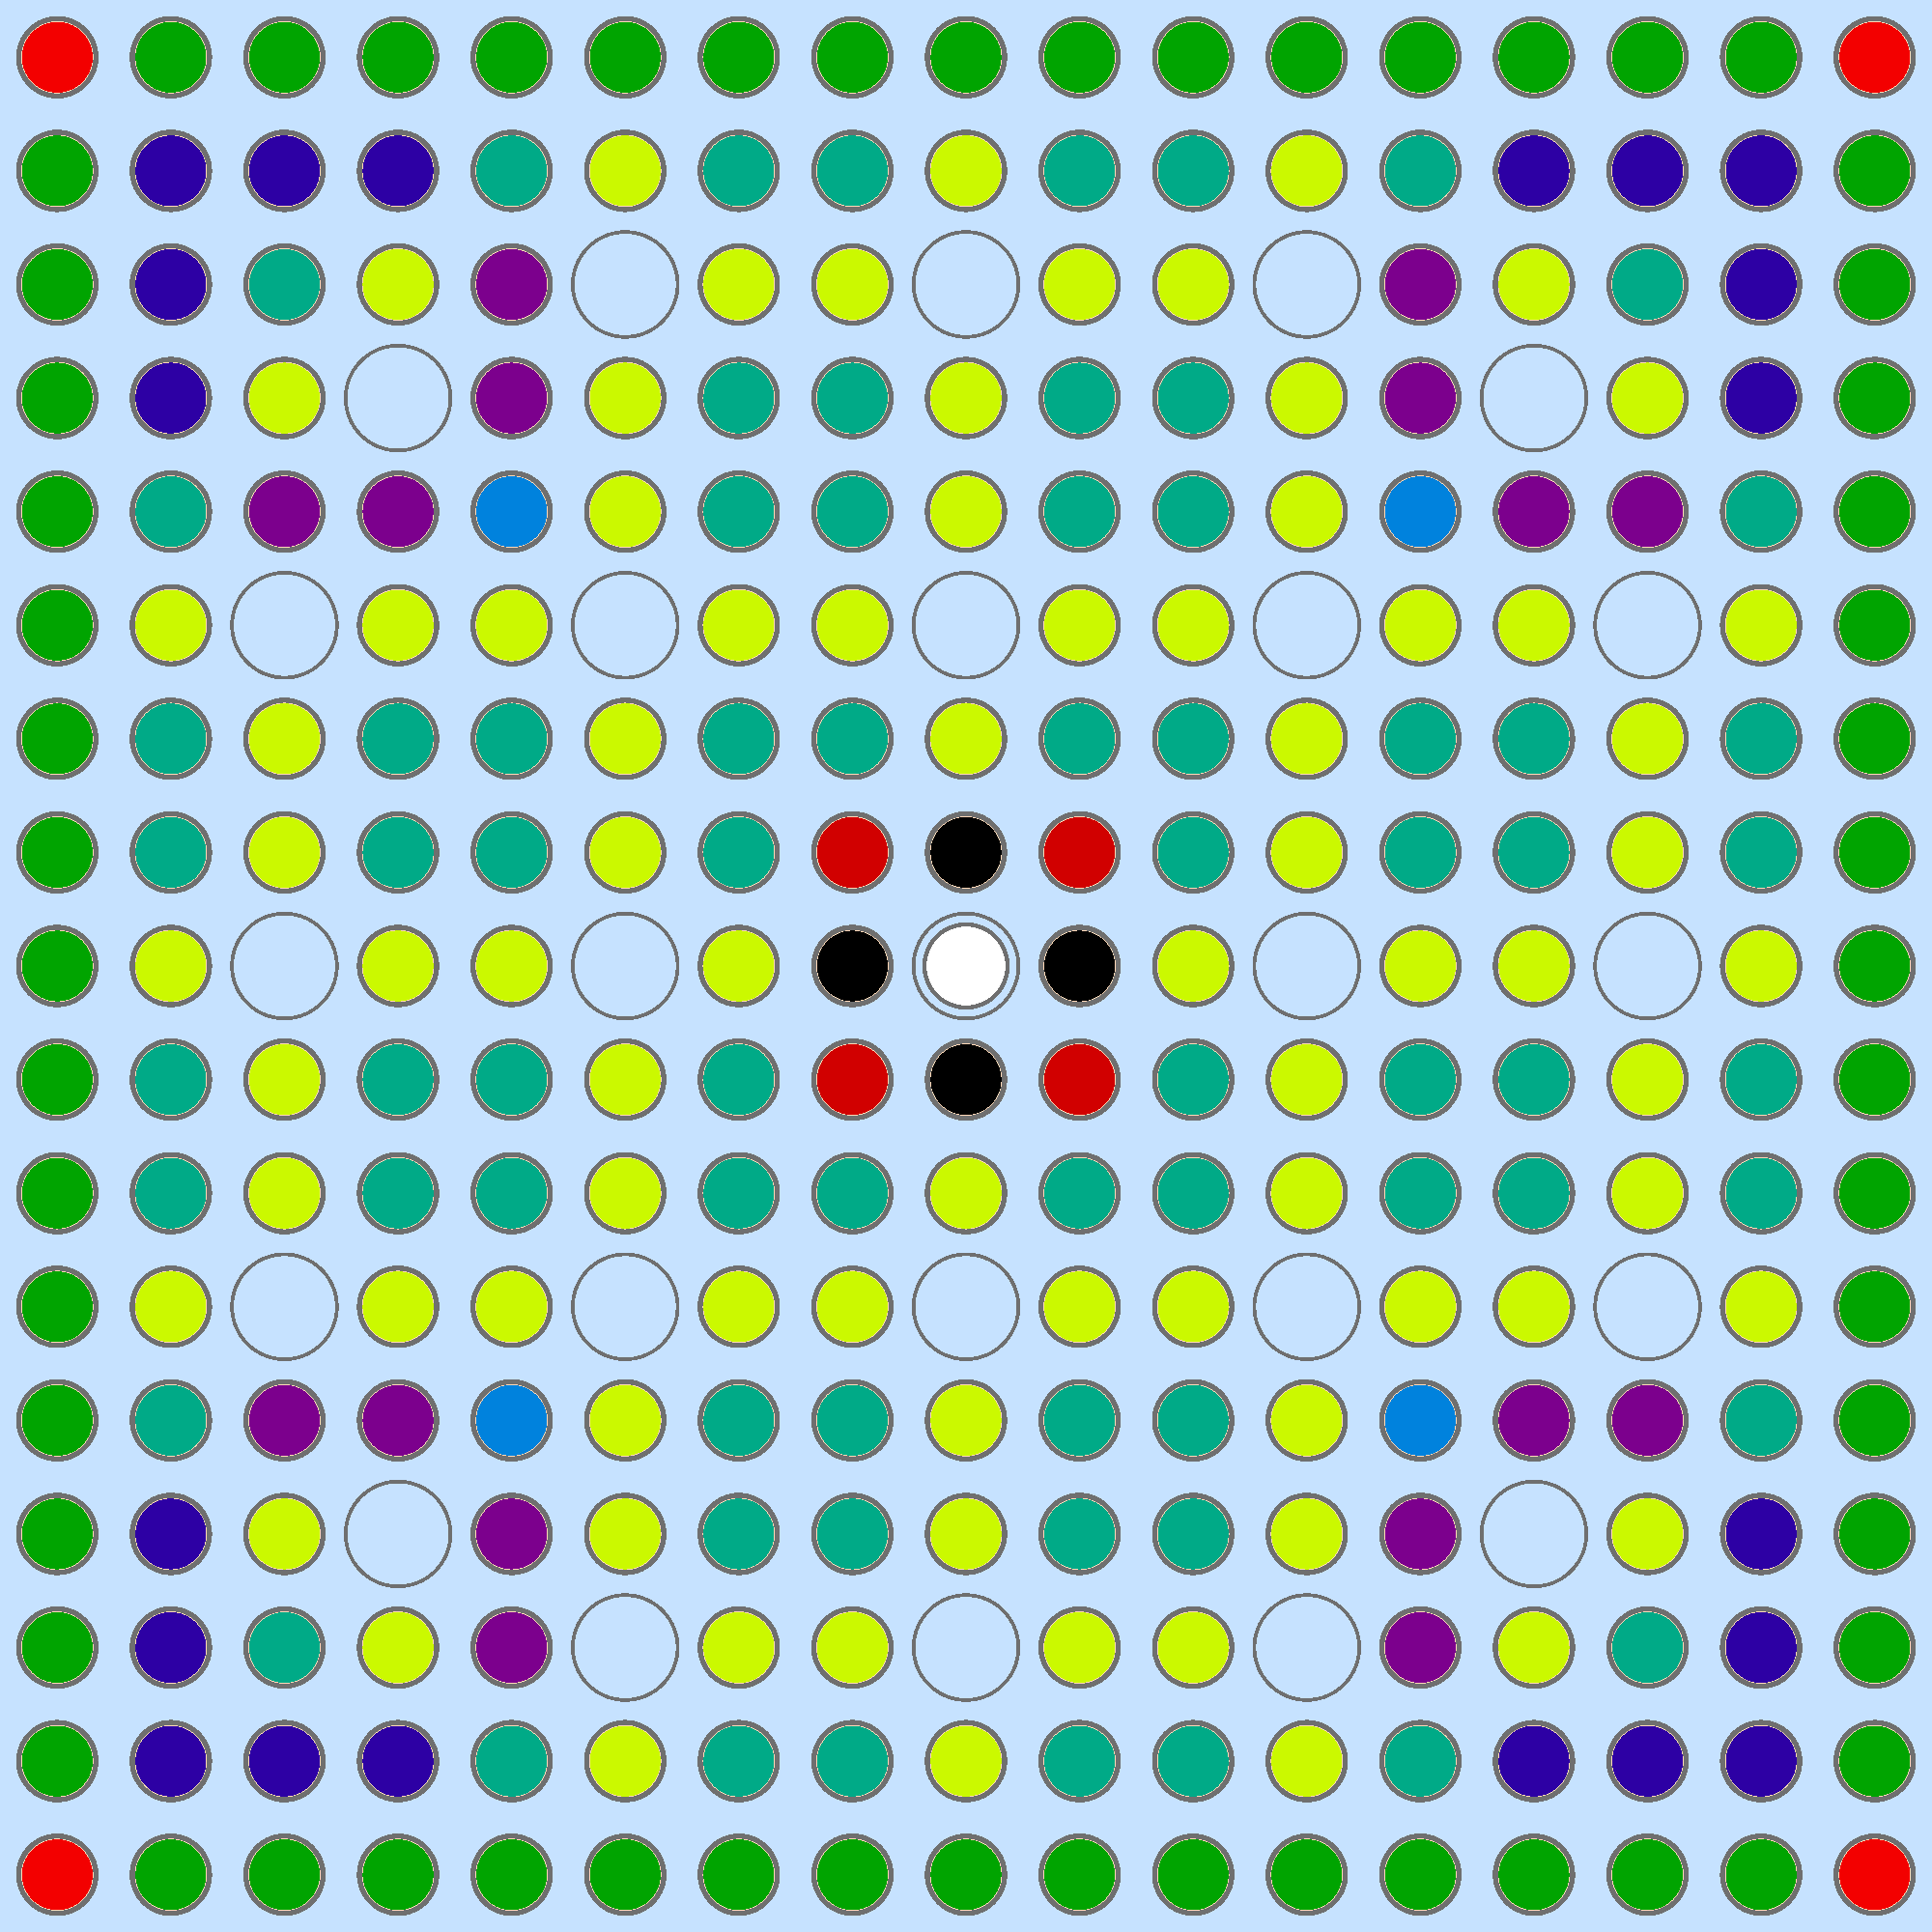
\includegraphics[width=0.9\linewidth]{figures/patterns/lns/assm-31/materials}
  \caption{}
  \label{fig:chap9-assm-31-lns-materials}
\end{subfigure}%
\begin{subfigure}{.47\textwidth}
  \centering
  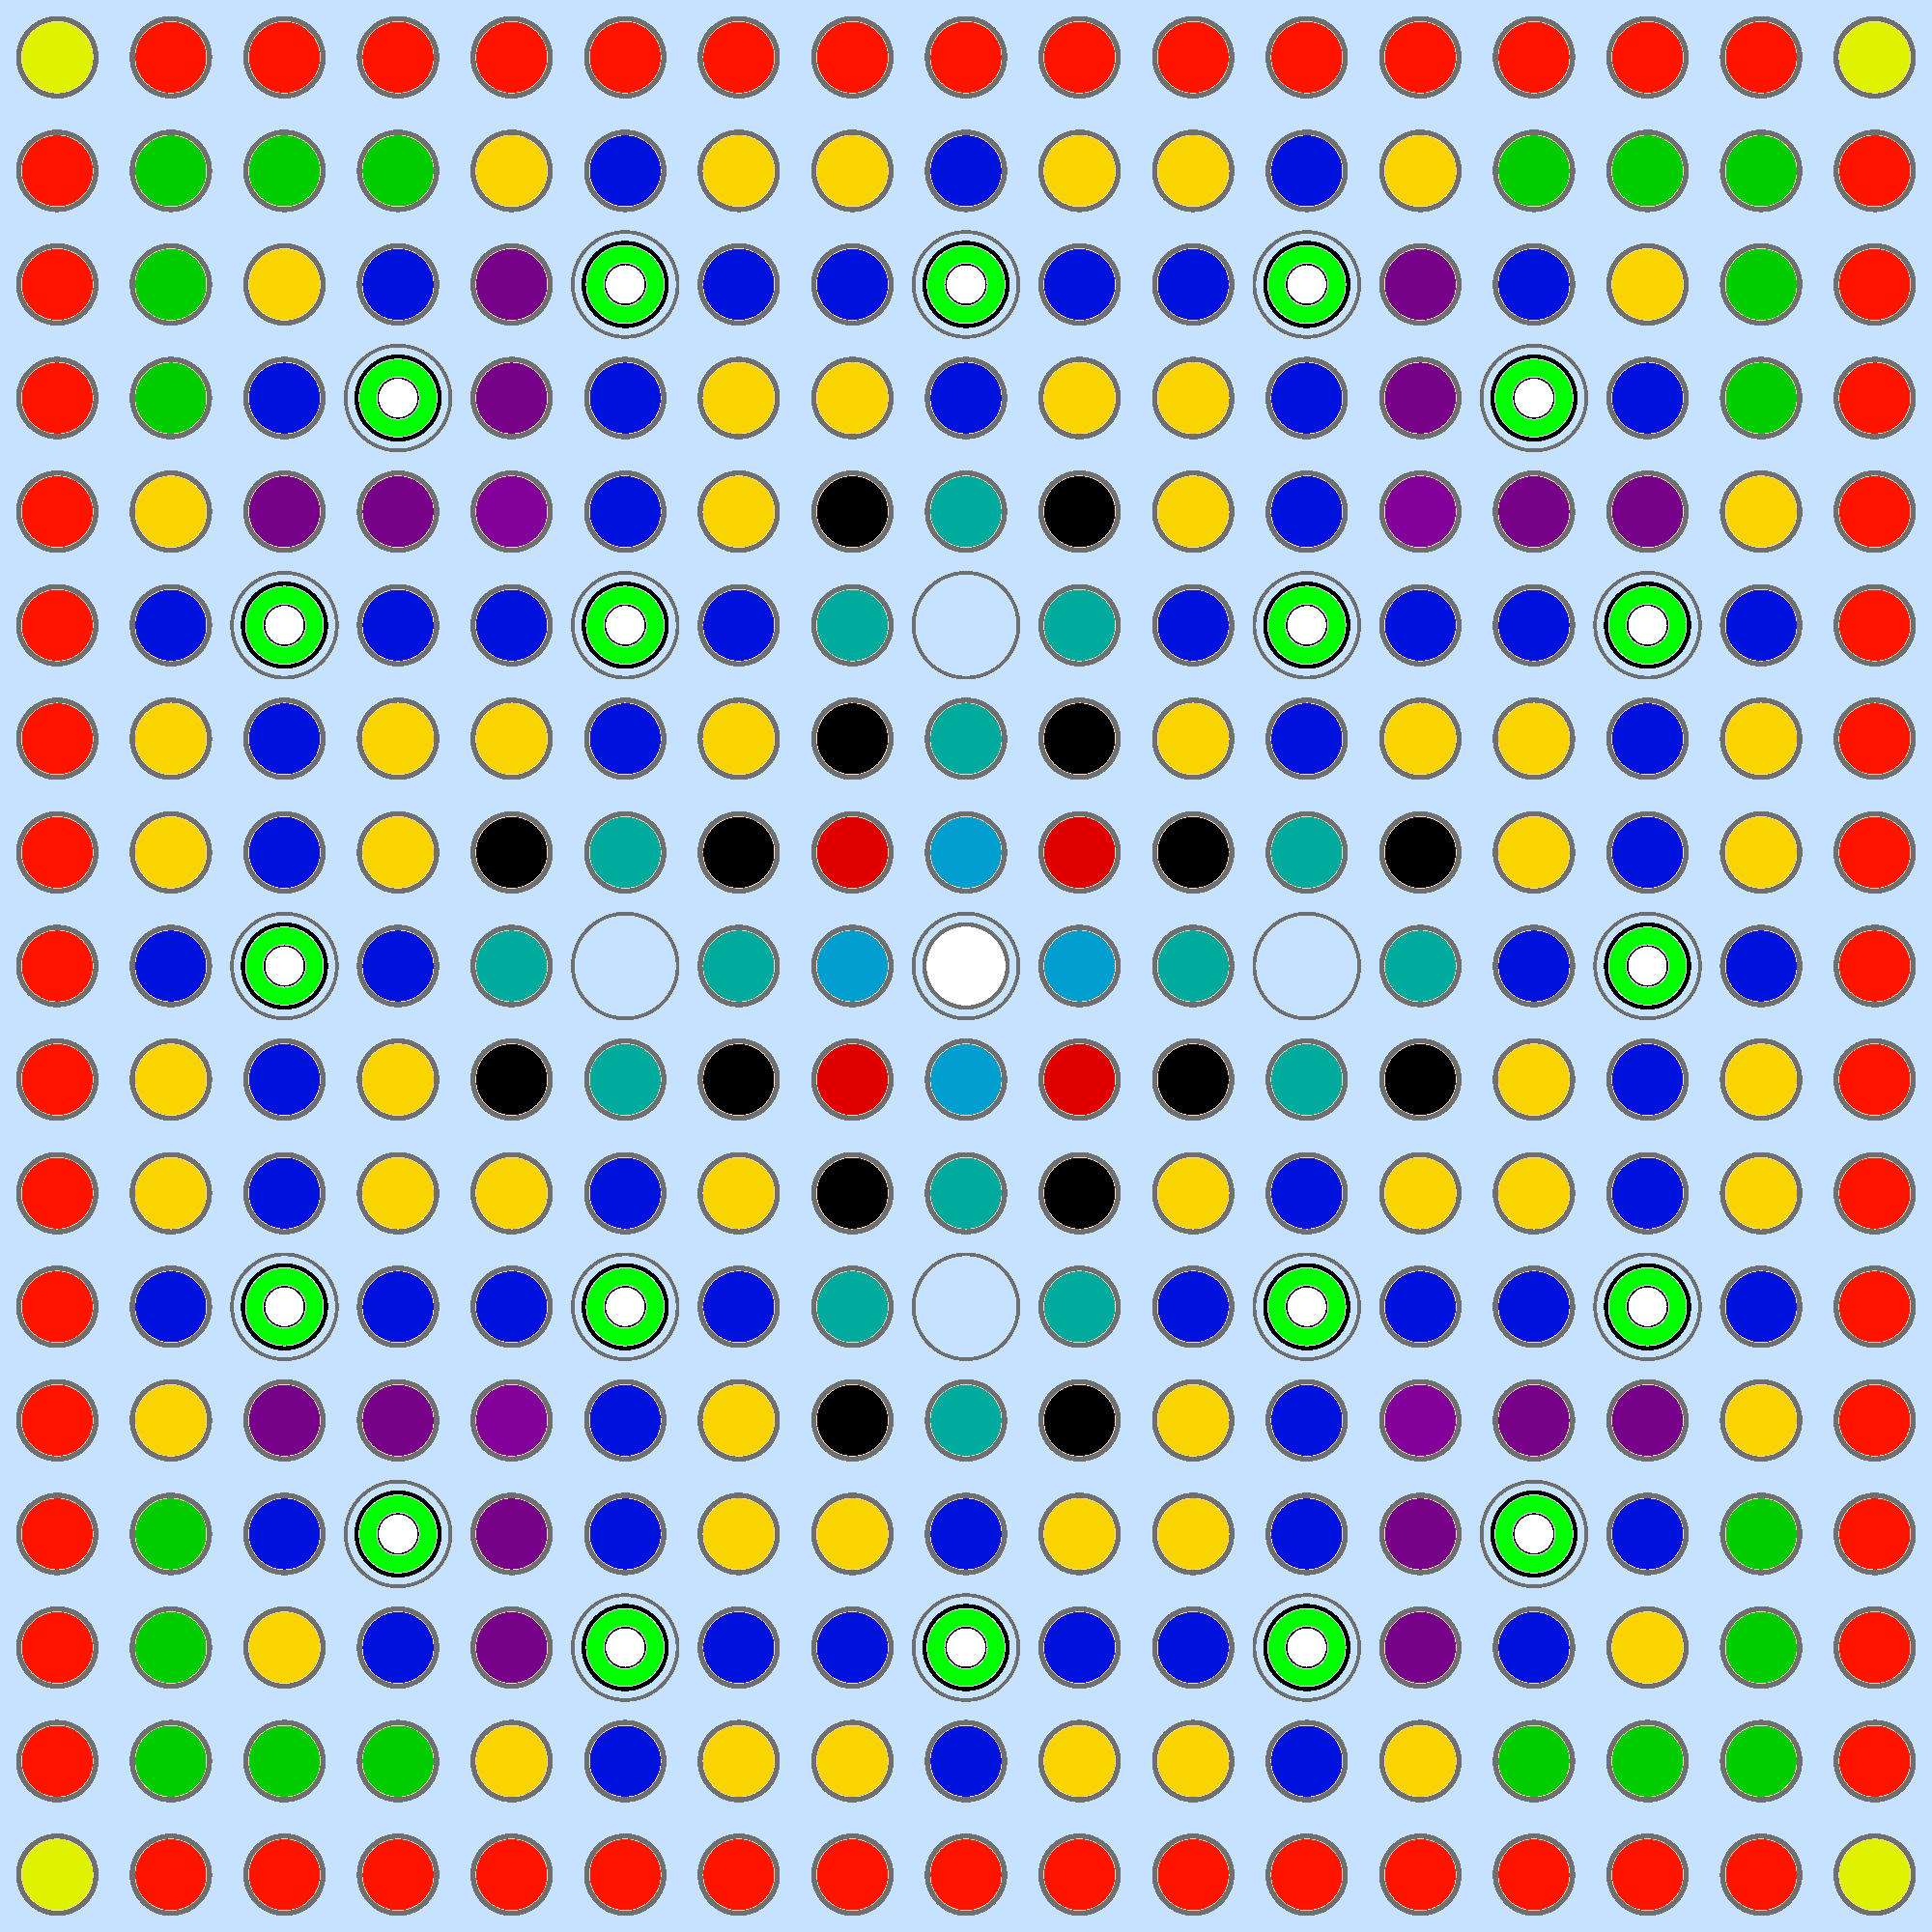
\includegraphics[width=0.9\linewidth]{figures/patterns/lns/assm-31-20BPs/materials}
  \caption{}
  \label{fig:chap9-31-20BPs-lns-materials}
\end{subfigure}
\begin{subfigure}{.47\textwidth}
  \centering
  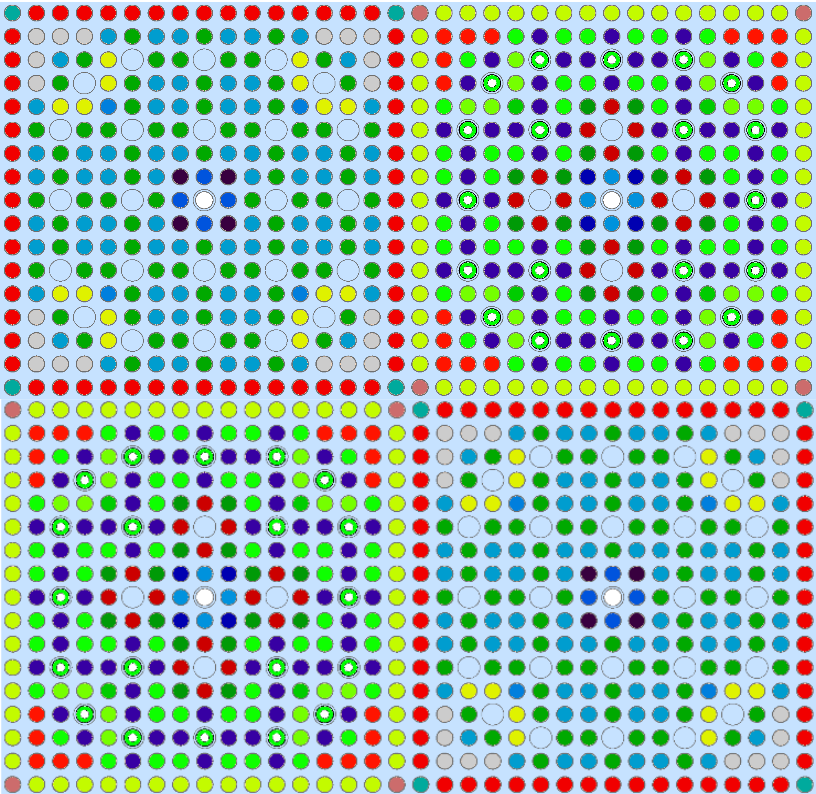
\includegraphics[width=0.9\linewidth]{figures/patterns/lns/2x2/materials}
  \caption{}
  \label{fig:chap9-2x2-lns-materials}
\end{subfigure}%
\begin{subfigure}{.47\textwidth}
  \centering
  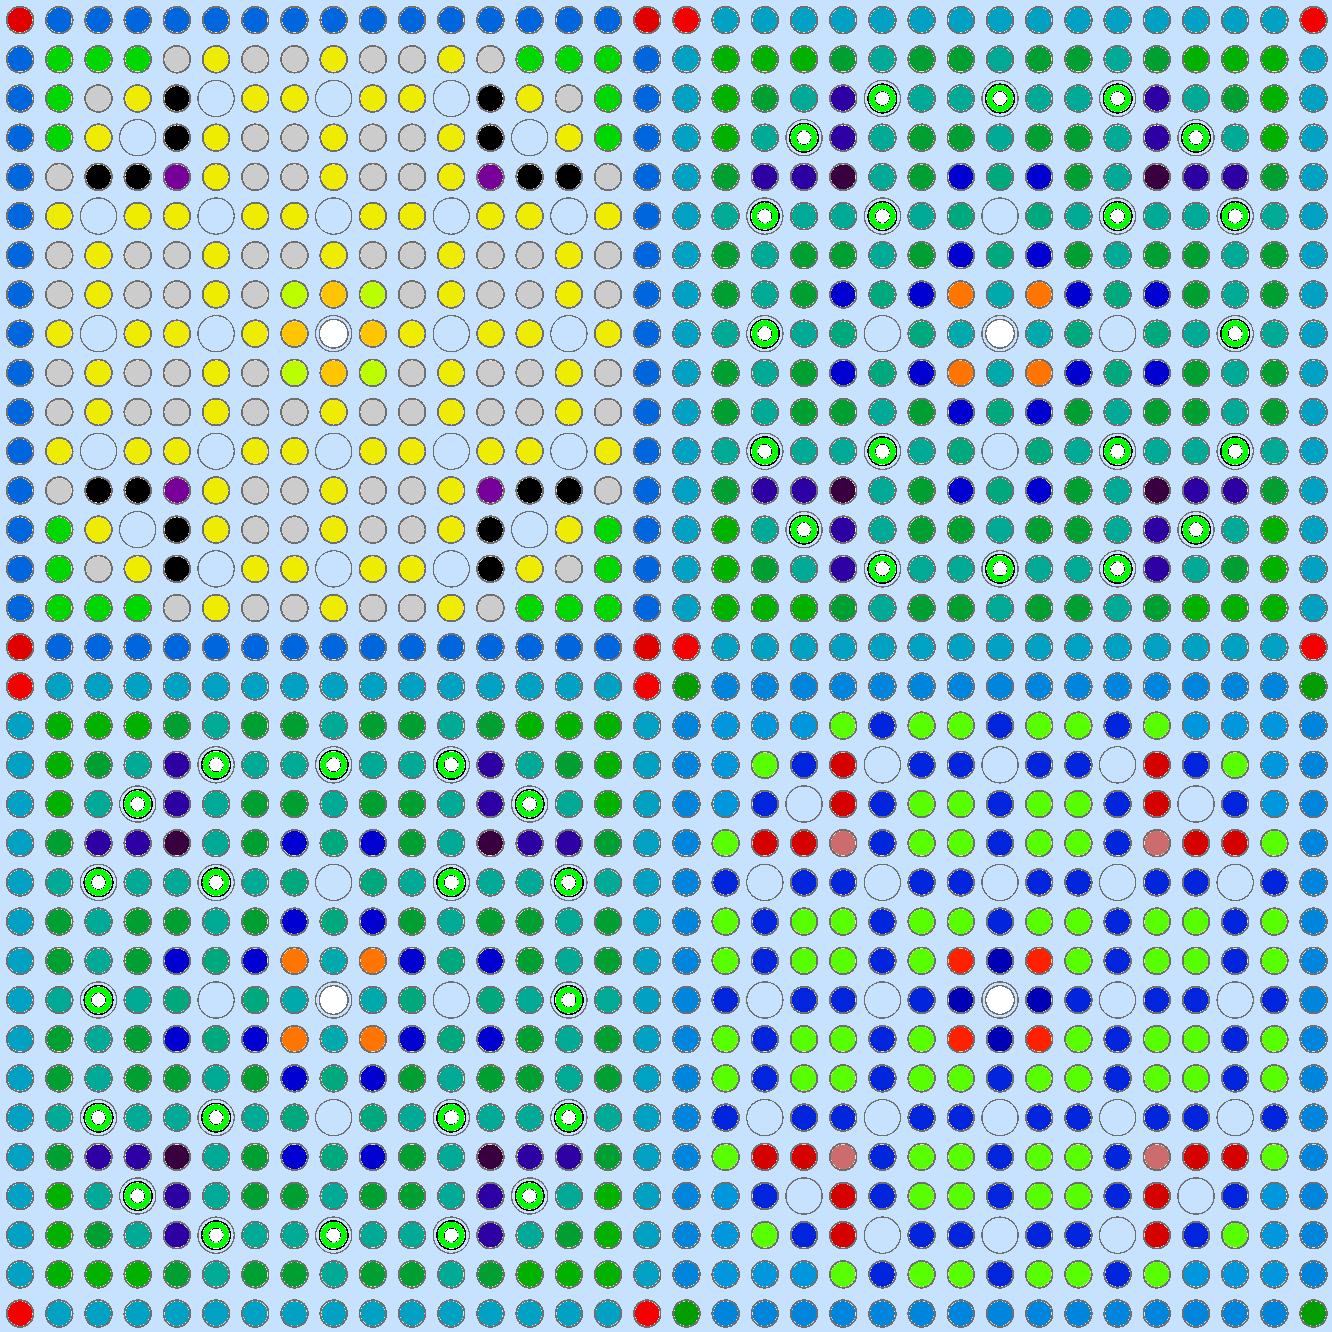
\includegraphics[width=0.9\linewidth]{figures/patterns/lns/reflector/materials}
  \caption{}
  \label{fig:chap9-reflector-lns-materials}
\end{subfigure}
\caption[Depiction of LNS spatially homogenized materials]{OpenMOC materials with \ac{LNS} spatial homogenization for a 1.6/3.1\% enriched fuel assembly (a), a 3.1\% enriched assembly with 20 \acp{BP} (b), a 2$\times$2 colorset without (c) and with (d) a reflector. Each uniquely colored material represents a unique set of \ac{MGXS}.}
\label{fig:chap9-lns-materials}
\end{figure}

\begin{figure}[h!]
\centering
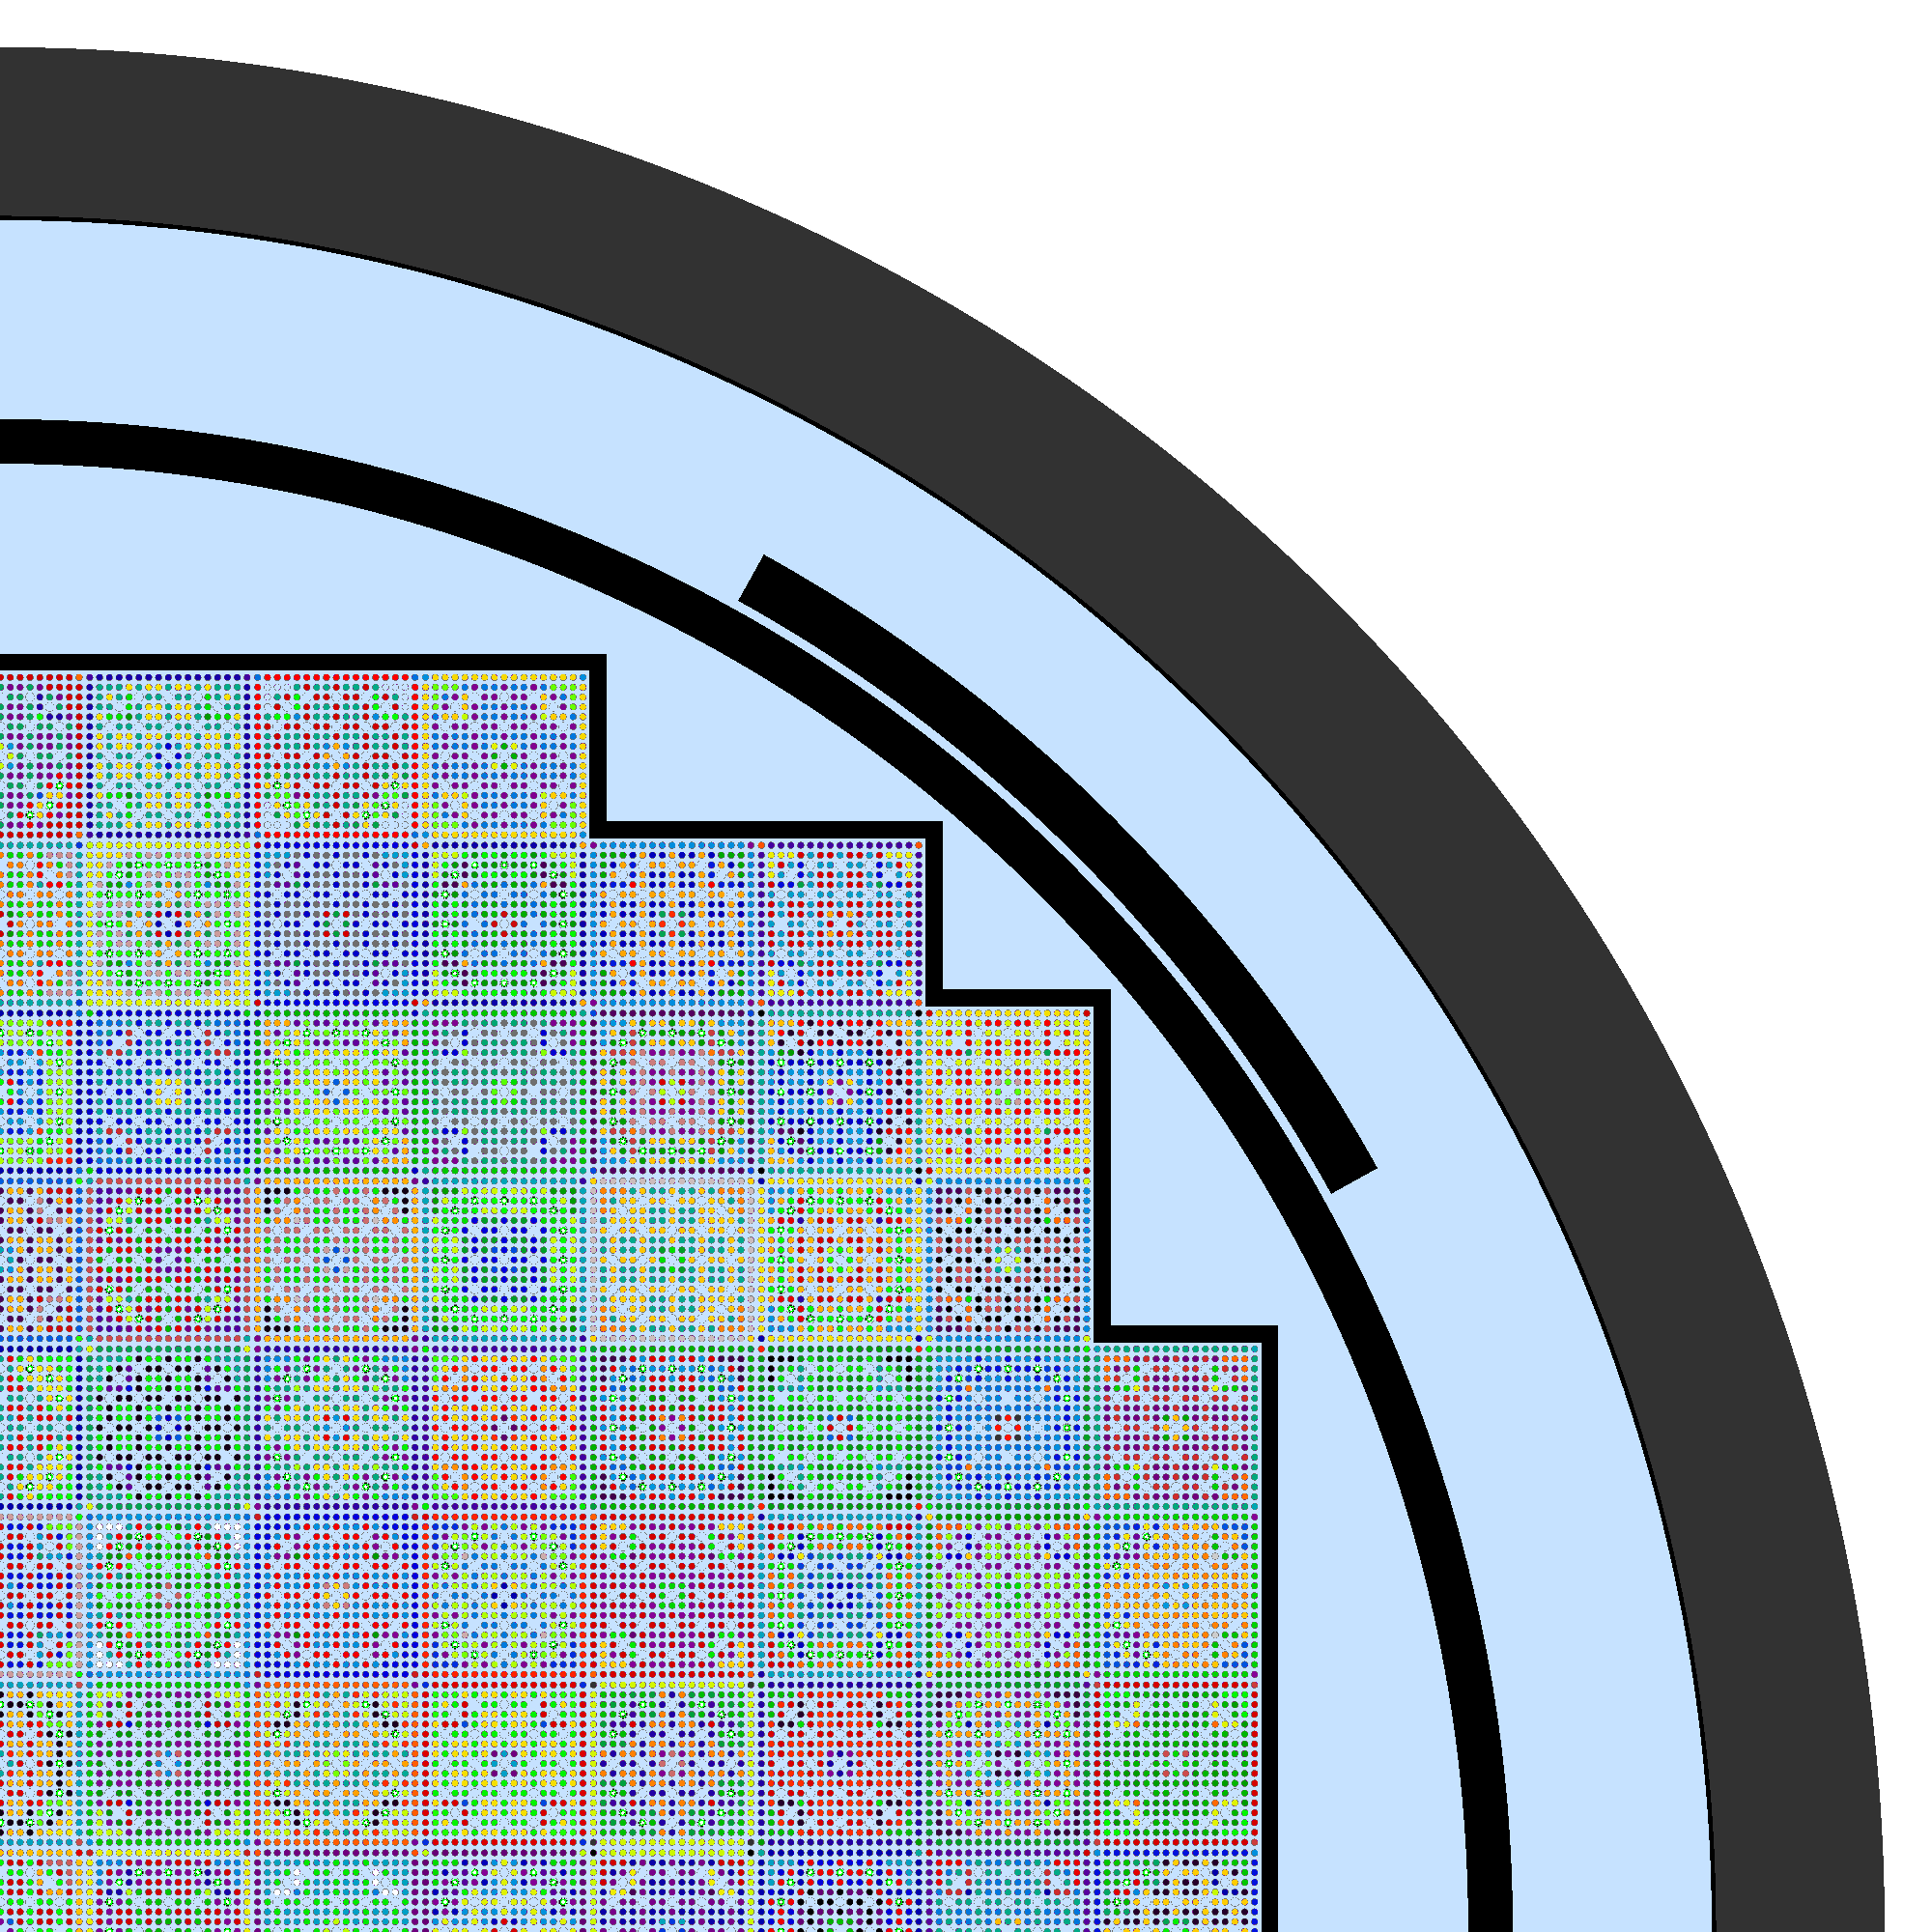
\includegraphics[width=\linewidth]{figures/patterns/lns/full-core/materials}
\caption{}
\caption[Depiction of LNS spatially homogenized materials for quarter core BEAVRS]{OpenMOC materials with \ac{LNS} spatial homogenization for the 2D quarter core \ac{BEAVRS} model. Each uniquely colored material represents a unique set of \ac{MGXS}.}
\label{fig:chap9-lns-materials-beavrs}
\end{figure}


\begin{table}[ht!]
  \centering
  \caption[OpenMOC eigenvalue bias with LNS homogenization]{OpenMOC eigenvalue bias $\Delta\rho$ for heterogeneous benchmarks with \ac{LNS} homogenization and varying energy group structures.}
  \small
  \label{table:chap9-lns-eigenvalues}
  \vspace{6pt}
  \begin{tabular}{l R{2.5cm} R{2.5cm} R{2.5cm}}
  \toprule
  \rowcolor{lightgray}
  & \multicolumn{3}{S[table-format=6.1]}{\cellcolor{lightgray} {$\bm{\Delta\rho}$ \textbf{[pcm]}}} \\
  \multirow{-2}{*}{\cellcolor{lightgray} \bf Benchmark} &
  \multicolumn{1}{r}{{\cellcolor{lightgray} \bf 2-Group}} &
  \multicolumn{1}{r}{{\cellcolor{lightgray} \bf 8-Group}} &
  \multicolumn{1}{r}{{\cellcolor{lightgray} \bf 70-Group}} \\
  \midrule
1.6\% Assm & -21 & -68 & -177 \\
3.1\% Assm & 33 & -67 & -211 \\
3.1\% Assm w/ 20 BPs & -115 & -166 & -267 \\
2$\times$2 Colorset & -63 & -159 & -270 \\
2$\times$2 Colorset w/ Reflector & 1873 & 525 & -112 \\
BEAVRS Full Core & & & \\
  \bottomrule
\end{tabular}
\end{table}

\begin{table}[ht!]
  \centering
  \caption[OpenMOC fission rate errors with LNS homogenization]{OpenMOC fission rate percent relative errors for heterogeneous benchmarks with \ac{LNS} spatial homogenization and varying energy group structures.}
  \small
  \label{table:chap9-lns-fiss-rates}
  \vspace{6pt}
  \begin{tabular}{l l R{2.5cm} R{2.5cm} R{2.5cm}}
  \toprule
  \rowcolor{lightgray}
  & & \multicolumn{3}{c}{\cellcolor{lightgray} \textbf{Error [\%]}} \\
  \multirow{-2}{*}{\cellcolor{lightgray} \bf Benchmark} &
  \multirow{-2}{*}{\cellcolor{lightgray} \bf Metric} &
  \multicolumn{1}{r}{{\cellcolor{lightgray} \bf 2-Group}} &
  \multicolumn{1}{r}{{\cellcolor{lightgray} \bf 8-Group}} &
  \multicolumn{1}{r}{{\cellcolor{lightgray} \bf 70-Group}} \\
  \midrule
\multirow{2}{*}{\parbox{2.2cm}{1.6\% Assm}} & Max & 2.048 & 0.735 & 0.353 \\
& Mean & 0.698 & 0.233 & 0.084 \\
\midrule
\multirow{2}{*}{\parbox{2.2cm}{3.1\% Assm}} & Max & 2.415 & 0.936 & 0.417 \\
& Mean & 0.826 & 0.298 & 0.094 \\
\midrule
\multirow{2}{*}{\parbox{2.2cm}{3.1\% Assm w/ 20 BPs}} & Max & -2.170 & -0.728 & 0.377 \\
& Mean & 0.785 & 0.219 & 0.096 \\
\midrule
\multirow{2}{*}{\parbox{2.2cm}{2$\times$2 Colorset}} & Max & -6.101 & -1.576 & 0.604 \\
& Mean & 3.283 & 0.751 & 0.163 \\
\midrule
\multirow{2}{*}{\parbox{2.2cm}{2$\times$2 Colorset w/ Reflector}} & Max & -14.515 & -2.937 & -0.785 \\
& Mean & 5.290 & 1.009 & 0.201 \\
\midrule
\multirow{2}{*}{\parbox{2.2cm}{BEAVRS Full Core}} & Max & & & \\
& Mean & & & \\
\bottomrule
\end{tabular}
\end{table}


\begin{table}[ht!]
  \centering
  \caption[OpenMOC U-238 capture rate errors with LNS homogenization]{OpenMOC U-238 capture rate percent relative errors for heterogeneous benchmarks with \ac{LNS} spatial homogenization and varying energy group structures.}
  \small
  \label{table:chap9-lns-capture-rates}
  \vspace{6pt}
  \begin{tabular}{l l R{2.5cm} R{2.5cm} R{2.5cm}}
  \toprule
  \rowcolor{lightgray}
  & & \multicolumn{3}{c}{\cellcolor{lightgray} \textbf{Error [\%]}} \\
  \multirow{-2}{*}{\cellcolor{lightgray} \bf Benchmark} &
  \multirow{-2}{*}{\cellcolor{lightgray} \bf Metric} &
  \multicolumn{1}{r}{{\cellcolor{lightgray} \bf 2-Group}} &
  \multicolumn{1}{r}{{\cellcolor{lightgray} \bf 8-Group}} &
  \multicolumn{1}{r}{{\cellcolor{lightgray} \bf 70-Group}} \\
  \midrule
\multirow{2}{*}{\parbox{2.2cm}{1.6\% Assm}} & Max & 1.088 & 0.450 & 0.304 \\
& Mean & 0.371 & 0.105 & 0.105 \\
\midrule
\multirow{2}{*}{\parbox{2.2cm}{3.1\% Assm}} & Max & 1.040 & 0.535 & 0.317 \\
& Mean & 0.389 & 0.120 & 0.104 \\
\midrule
\multirow{2}{*}{\parbox{2.2cm}{3.1\% Assm w/ 20 BPs}} & Max & 1.898 & 0.781 & 0.418 \\
& Mean & 0.510 & 0.176 & 0.105 \\
\midrule
\multirow{2}{*}{\parbox{2.2cm}{2$\times$2 Colorset}} & Max & 3.038 & -0.765 & -0.780 \\
& Mean & 1.541 & 0.202 & 0.193 \\
\midrule
\multirow{2}{*}{\parbox{2.2cm}{2$\times$2 Colorset w/ Reflector}} & Max & 8.766 & 3.733 & 2.592 \\
& Mean & 3.444 & 0.558 & 0.301 \\
\midrule
\multirow{2}{*}{\parbox{2.2cm}{BEAVRS Quarter Core}} & Max & & & \\
& Mean & & & \\
\bottomrule
\end{tabular}
\end{table}


\begin{figure}[h!]
\centering
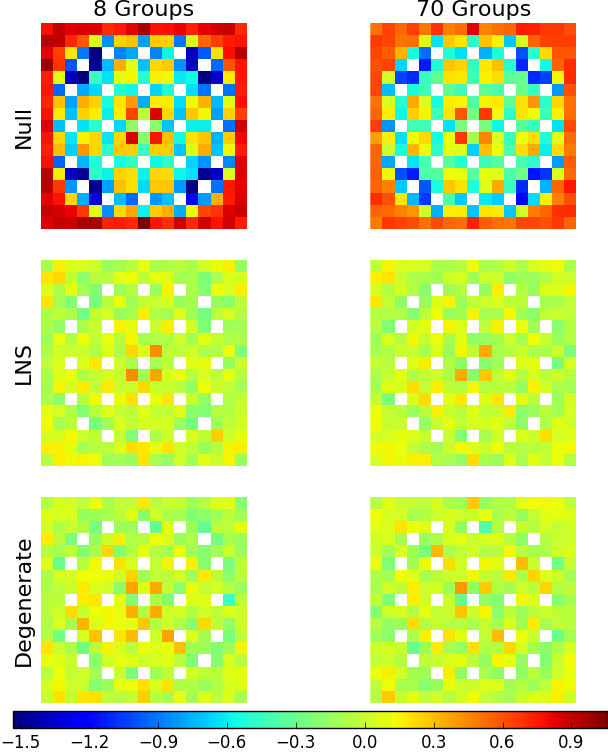
\includegraphics[width=\linewidth]{figures/patterns/lns/assm-16/capt-err}
\vspace{2mm}
\caption[U-238 capture rate errors for a 1.6\% enriched assembly]{U-238 capture rate percent relative errors errors for a 1.6\% enriched assembly with \ac{LNS} spatial homogenization.}
\label{fig:chap9-assm-1.6-lns-capt-err}
\end{figure}

\clearpage

\begin{figure}[h!]
\centering
\includegraphics[width=\linewidth]{figures/patterns/lns/assm-31/capt-err}
\vspace{2mm}
\caption[U-238 capture rate errors for a 3.1\% enriched assembly]{U-238 capture rate percent relative errors errors for a 3.1\% enriched assembly with \ac{LNS} spatial homogenization.}
\label{fig:chap9-assm-3.1-lns-capt-err}
\end{figure}

\clearpage

\begin{figure}[h!]
\centering
\includegraphics[width=\linewidth]{figures/patterns/lns/assm-31-20BPs/capt-err}
\vspace{2mm}
\caption[U-238 capture rate errors for a 3.1\% enriched assembly with 20 BPs]{U-238 capture rate percent relative errors errors for a 3.1\% enriched assembly with 20 \acp{BP} with \ac{LNS} spatial homogenization.}
\label{fig:chap9-assm-3.1-20BPs-lns-capt-err}
\end{figure}

\clearpage

\begin{figure}[h!]
\centering
\includegraphics[width=\linewidth]{figures/patterns/lns/2x2/capt-err}
\vspace{2mm}
\caption[U-238 capture rate errors for a 2$\times$2 colorset]{U-238 capture rate percent relative errors errors for a 2$\times$2 colorset with \ac{LNS} spatial homogenization.}
\label{fig:chap9-2x2-lns-capt-err}
\end{figure}

\clearpage

\begin{figure}[h!]
\centering
\includegraphics[width=\linewidth]{figures/patterns/lns/reflector/capt-err}
\vspace{2mm}
\caption[U-238 capture rate errors for a 2$\times$2 colorset with a reflector]{U-238 capture percent relative errors rate errors for a 2$\times$2 colorset with \ac{LNS} spatial homogenization.}
\label{fig:chap9-reflector-lns-capt-err}
\end{figure}

\clearpage

%\begin{figure}[h!]
%\centering
%\includegraphics[width=\linewidth]{figures/patterns/lns/full-core/capt-err}
%\vspace{2mm}
%\caption[U-238 capture rate errors for the 2D quarter core \ac{BEAVRS} model]{U-238 capture percent relative errors rate errors for the 2D quarter core \ac{BEAVRS} model corresponding to the reference in Fig.~\ref{fig:chap7-capt-rates-full-core}.}
%\label{fig:chap8-full-core-capt-err}
%\end{figure}

\clearpage


\begin{figure}[h!]
\centering
\begin{subfigure}{.87\textwidth}
  \centering
  \includegraphics[width=\linewidth]{figures/patterns/convergence/assm-16/assm-16-capt}
  \caption{}
  \label{fig:chap9-assm-16-converge}
\end{subfigure}
\begin{subfigure}{.87\textwidth}
  \centering
  \includegraphics[width=\linewidth]{figures/patterns/convergence/full-core/16-enr-capt}
  \caption{}
  \label{fig:chap9-reflector-converge}
\end{subfigure}
\caption[Convergence of pin-wise U-238 capture MGXS]{The batch-wise change of pin-wise U-238 capture \ac{MGXS} (group 27 of 70) for 1.6\% enriched fuel pins in a single assembly (a) and the quarter core \ac{BEAVRS} model (b). The convergence of both the maximum and mean absolute percent change are shown for the degenerate and \ac{LNS} homogenization schemes.}
\label{fig:chap9-converge}
\end{figure}
